% !TEX root = mythesis.tex



%==============================================================================
\chapter{ABCD data-driven method}
\label{sec:abcd}
%==============================================================================
The goal of this chapter is to introduce one of the data-driven methods called the ABCD method, which is used to estimate multijet in this analysis. An overview of how a correction is applied to the results from the ABCD method, which leads to an introduction of the correction factor is given. Four different approaches of calculation of the correction factor are discussed in the last section of this chapter.

%==============================================================================
\section{Data-driven estimation of background}
\label{sec:abcd:data-driven}
%==============================================================================
Sometimes it is difficult to simulate a background process very precisely using the MC production because of several reasons. For example, limited understanding of the QCD process, inability to simulate hadronisation with precision, need large MC samples to simulate all the possible cases, not sufficient computing power, not an accurate understanding of all details in the detector and also when uncertainties from the simulation are significant or not known. So, one needs an alternative way of producing these background processes. The alternative approach is the extraction of background from the experimental data itself in a combination of the MC simulation. This technique is known as a data-driven method. Some standard data-driven methods are matrix method, ABCD method and the fake factor method. In this thesis, the ABCD method is used to estimate the multijet background, which is discussed in detail in the next section.

%==============================================================================
\section{The ABCD method}
\label{sec:abcd:method}
%==============================================================================
The ABCD method is generally used to estimate the backgrounds which are difficult to understand from the MC simulation. The idea behind this method is first to choose two uncorrelated variables, which means two mutually independent variables that can characterise the data in order to estimate the background. After that, four mutually exclusive regions are defined by making selections on these two variables. These regions are defined in such a way that one of the regions should be enriched in signal events where the contribution from the background events should be low. The other three regions should be signal-deficient regions where the background events should be in excess.~\cite{thesis:arshia}

\begin{figure}[hbt!]
	\centering
	\includegraphics[width=0.5\linewidth]{abcd.png}
	\caption{A pictorial representation of the ABCD method where four regions A, B, C and D are defined by the selections made on two orthogonal variables x and y. Region A (in grey) is a signal-enriched region and the other three regions (in white) are signal-deficient regions.}
	\label{fig:abcd:method}
\end{figure}

A schematic for visualisation is given in Fig.\ \ref{fig:abcd:method}, which shows two-dimensional phase space spanned by two uncorrelated variables x and y. Region A, B, C and D are defined in a manner such that region A is a signal-enriched region (where the background estimate has to be performed) and region B, C and D are signal-deficient regions. Then, the background estimate in region A can be estimated by extrapolating the background events from the signal-deficient regions by Eqn.\ \ref{eqn:abcd:method}:

\begin{equation}
	N_{\text{A}} = N_{\text{B}} \times \frac{N_{\text{D}}}{N_{\text{C}}} \,,
	\label{eqn:abcd:method}
\end{equation}
where $N_{\text{j}}$ denotes the number of background events in region j $\in$ \{A,B,C,D\}.

\subsubsection{Assumptions:}
There are some assumptions to the ABCD method, which need to be fulfilled before implementing the method to the data. The important assumptions are discussed in detail below:

\begin{enumerate}
	\item The two variables x and y should be chosen in such a way that they are perfectly uncorrelated.
	
	\item The foundation of this method relies on the definition of the regions. The signal-deficient regions should not contain any signal events. The signal contamination can be examined by calculating the signal-background ratio in all the regions. It is calculated by~\cite{signalbackgroundratio}: 
	\begin{equation}
		\text{Signal-background ratio = } \sqrt{2\left[(N_{\text{j}}^{\text{S}}+N_{\text{j}}^{\text{B}})\ln(1+\frac{N_{\text{j}}^{\text{S}}}{N_{\text{j}}^{\text{B}}})-N_{\text{j}}^{\text{S}}\right]} \approx \frac{N_{\text{j}}^{\text{S}}} {\sqrt{N_{\text{j}}^{\text{B}}}} \,,
		\label{eqn:abcd:sbratio}
	\end{equation}
	 where $N_{\text{j}}^{\text{S}}$ and $N_{\text{j}}^{\text{B}}$ denote the number of signal and background MC events respectively in region j $\in$ \{A,B,C,D\}.
	
	\item Since it is a data-driven method, so there should be enough data events in the signal-deficient regions to extrapolate the background behaviour precisely to region A. It is also useful to propagate the statistical uncertainty on the background estimate in region A.
	
\end{enumerate}


%==============================================================================
\section{Implementation of the ABCD method}
\label{sec:abcd:implementation}
%==============================================================================

%==============================================================================
\subsection{Choice of variables}
\label{sec:abcd:implementation:variables}
%==============================================================================
In this thesis, the ABCD method is used to estimate the multijet background. So, it is important to choose variables that ensure abundance of the multijet background in signal-deficient regions. The variables $W$-tagging efficiency and the $b$-jet multiplicity are chosen because according to one of the assumptions, the two variables should be perfectly uncorrelated. In $W$-tagging, it is explicitly made sure that no $b$-tagging information is used. Thus, choosing them as two uncorrelated variables for the ABCD method. 

The working point efficiency of $W$-tagging is chosen as one of the variables for the ABCD method. The two selected working points (WP) are $80\%$ referred as $loose$, and $50\%$ referred as $tight$. Tight is a subset of loose because it has a stronger criteria and therefore, less number of events have large-$R$ jets which pass tight $W$-tagging criteria. The three regions which are defined by making the selections based on these two working points are tight, loose not tight, and not loose. These regions are described in detail below:
\begin{itemize}
	\item Tight: it contains events which have large-$R$ jets that are $W$-tagged at 50\% WP.
	\item Loose not tight: it contains events which have large-$R$ jets that are $W$-tagged at 80\% WP but not tagged at 50\%.
	\item Not loose: it contains all the events which have large-$R$ jets that are not $W$-tagged at 80\% WP. 
\end{itemize}
There are two taggers for large-$R$ jets which are used in this thesis, i.e.\ two-variable tagger and three-variable tagger. In this chapter, large-$R$ jets which are tagged with three-variable tagger are used for the estimation of multijet background using the ABCD method. The estimation with two-variable tagger is also performed and used to compare the performance of the two taggers, which are described in section \ref{sec:results:taggers}.

The presence of $b$-jets can further characterise the signal and background events. So the multiplicity of $b$-tagged jets is chosen as the second variable. The two regions which are defined based on this are $0b$ and $\geq1b$, which are described in detail below:
\begin{itemize}
\item $0b$: it contains events which do not have any small-$R$ jets that are $b$-tagged.
\item $\geq1b$: it contains events which have at least one small-$R$ jet that is $b$-tagged.
\end{itemize}
There are two jet collections for small-$R$ jets which are used in this thesis, i.e.\ EMTopo and PFlow jets. In this chapter, PFlow jet collection is used for the estimation of multijet background using the ABCD method. The estimation with EMTopo jet collection is also performed and used to compare the performance of the two jet collections, which are described in section \ref{sec:results:jetcollections}.

%==============================================================================
\subsection{Definition of regions}
\label{sec:abcd:implementation:regions}
%==============================================================================
There are six regions which are defined by making selection cuts on these two variables. A pictorial representation is shown in Fig.\ \ref{fig:abcd:method:regions}. It shows $b$-jet multiplicity on the x-axis and $W$-tagging WP on the y-axis. The regions include signal region, validation region and control region, which are described in detail below:

\begin{figure}[hbt!]
	\centering
	\includegraphics[width=0.8\linewidth]{abcd_regions.png}
	\caption{A representation of all the ABCD regions defined on two uncorrelated variables. Region A1 is signal region, region A is validation region and the other four regions B, C, D, D1 are control regions.}
	\label{fig:abcd:method:regions}
\end{figure}

%==============================================================================
\subsubsection{Signal region}
\label{sec:abcd:implementation:regions:sr}
%==============================================================================
Signal region (SR) is defined in such a way that it should be enriched with signal events. Region A1 is represented as SR, which should contain those events which pass the following criteria. The leading large-$R$ jet should be $W$-tagged at tight selection. Along with that, the events should have at least one $b$-tagged jet, and the leading $b$-tagged jet (denoted by $b_{\text{1}}$) should be a central jet which means it should lie within the central region of the detector which can be made sure by $|\eta_{b_{1}}| < 2.5$ cut. Also, the leading $b$-tagged jet should not be a part of $W$-tagged large-$R$ jet and should be well separated which is ensured by implementing $\Delta R(W,b_{\text{1}}) > 1.0$ cut. It was observed that after applying this cut, many events were filtered out because there were so many $b$-tagged jets inside the $W$-tagged large-$R$ jet. In this analysis, data is blinded in SR, which means all the calculations in this region can only be performed by using the MC samples.

%==============================================================================
\subsubsection{Validation region}
\label{sec:abcd:implementation:regions:vr}
%==============================================================================
Validation region (VR) is defined in such a way that kinematically it is close to the SR but not exactly the SR. So, region A is represented as VR to check and validate the method. VR includes selection cuts in which method can be applied both to the data and MC without exploiting the fact that it is biased to the SR. The selection cuts include leading large-$R$ jet to be $W$-tagged at loose not tight selection with a requirement of at least one $b$-tagged jet, where the leading $b$-tagged jet lies in a central region of the detector. The $\Delta R(W,b_{\text{1}}) > 1.0$ is also implemented to remove the events where the $W$-tagged jet and $b$-jets are not well separated. Multijet estimation is performed in VR using the ABCD method, and the data/bkg.\ comparison plots are shown to understand how well the estimation agrees with the data.

%==============================================================================
\subsubsection{Control region}
\label{sec:abcd:implementation:regions:cr}
%==============================================================================
Control region (CR) is defined in such a way that it should be enriched with background events. Region B, C, D, and D1 are referred to as CR. The selection cuts for all the four CRs are described in detail below:

\begin{itemize}
	\item \textbf{Region B:} it consists of the events which should at least have a large-$R$ jet, and the leading large-$R$ jet should not be $W$-tagged at the loose selection. Events should also have at least one $b$-tagged jet, where the leading $b$-tagged jet lies in a central region of the detector. The leading large-$R$ jet and the leading $b$-tagged jet should be well separated by imposing the condition $\Delta R(J_{\text{1}},b_{\text{1}}) > 1.0$, where $J_{\text{1}}$ is defined as the leading large-$R$ jet.
	
	\item \textbf{Regions C, D and D1:} all the three regions contain events in which none of the small-$R$ jets is $b$-tagged and the leading small-$R$ jet (denoted by $j_{\text{1}}$) should be a central jet. The selection cut which distinguishes the events in these three regions is the requirement of leading large-$R$ jet not to be $W$-tagged in the case of region C, and $W$-tagged at tight and loose not tight selection in the case of region D and D1 respectively. Furthermore, the leading large-$R$ jet (whether $W$-tagged or not) and the leading small-$R$ jet should be well separated by imposing a condition on $\Delta R(W/J_{\text{1}},j_{\text{1}}) > 1.0$.
\end{itemize}

%==============================================================================
\subsection{Closure tests}
\label{sec:abcd:implementation:closuretests}
%==============================================================================
Before proceeding with the estimation of the multijet background using the ABCD method, two preliminary closure tests are performed to check whether the defined regions are consistent with the assumptions. These are described in detail below: 

%==============================================================================
\subsubsection{Test I}
\label{sec:abcd:implementation:closuretests:testi}
%==============================================================================
The ABCD method is based on the assumption that the regions should be defined in such a way that the CRs should not have any signal events. In order to look at this, the MC signal samples are chosen, and the event yields are evaluated in all the six regions. This test is performed on the samples with different coupling values keeping the VLQ mass fixed, and also on the samples with different VLQ masses, keeping the coupling values constant. This is to make sure that the test is not biased to any mass and coupling values of the signal sample. So, four different MC signal samples are considered, which are shown in Table \ref{table:abcd:implementation:closuretests:testi:samples}.
\begin{table}[hbt!]
	\centering
	\begin{tabular}{c|c|c} 
		\toprule
		\textbf{Sample} & \textbf{VLQ mass} & \textbf{$k_\text{T}$} \\
		\midrule
		I & \SI{1.1}{\tera\electronvolt} & 0.1 \\
		II & \SI{1.5}{\tera\electronvolt} & 0.1 \\
		III & \SI{1.1}{\tera\electronvolt} & 0.3 \\
		IV & \SI{1.5}{\tera\electronvolt} & 0.3 \\
		\bottomrule
	\end{tabular}
	\caption{Four different MC signal samples along with their mass and coupling values which are used in closure test I. }
	\label{table:abcd:implementation:closuretests:testi:samples}
\end{table}

Table \ref{table:abcd:implementation:closuretests:testi} shows the event yields of the MC samples of all the backgrounds and the four MC simulated signal samples in all the six ABCD regions. Note that the multijet MC samples are the ones which are mismodelled. The event yield from the multijet MC samples is used to calculate the signal-background ratio, which is defined by Eqn.\ \ref{eqn:abcd:sbratio}, where $N^{\text{B}}_{\text{j}}$ is total background events from MC samples which are shown in Table \ref{table:abcd:implementation:closuretests:testi}. Fig.\ \ref{fig:abcd:implementation:closuretests:testi} shows the signal-background ratio for all the four signal samples. It can be observed in these plots that the choice of region A1 and A are in such a way that they are enriched in signal events, and the signal contamination in other regions (CRs) are negligible. So, the choice of the selection cuts to define these regions fulfill one of the main assumptions of the ABCD method.


\begin{sidewaystable}[!htbp]
		\centering
		\begin{tabular}{ c | c | c | c | c | c | c } 
			\toprule
			MC sample & SR & VR & \multicolumn{4}{c}{CR} \\ \cline{2-7}
			& Region A1 & Region A & Region B & Region C & Region D & Region D1 \\
			\midrule
			Single top & $\num{1130}\pm\num{18}$ & $\num{714}\pm\num{14}$ & $\num{861}\pm\num{15}$ & $\num{165}\pm\num{7}$ & $\num{9}\pm\num{1}$ & $\num{14}\pm\num{2}$ \\
			$t\bar{t}$ & $\num{568}\pm\num{14}$ & $\num{964}\pm\num{19}$ & $\num{5614}\pm\num{45}$ & $\num{894}\pm\num{18}$ & $\num{25}\pm\num{3}$ & $\num{15}\pm\num{2}$ \\
			$W$+jets & $\num{1257}\pm\num{80}$ & $\num{1022}\pm\num{82}$ & $\num{3937}\pm\num{178}$ & $\num{7627}\pm\num{234}$ & $\num{1540}\pm\num{94}$ & $\num{1991}\pm\num{109}$ \\
			$Z$+jets & $\num{317}\pm\num{27}$ & $\num{617}\pm\num{42}$ & $\num{4264}\pm\num{125}$ & $\num{2648}\pm\num{88}$ & $\num{744}\pm\num{43}$ & $\num{496}\pm\num{34}$ \\
			Multijet & $\num{15726}\pm\num{343}$ & $\num{75607}\pm\num{738}$ & $\num{395532}\pm\num{1667}$ & $\num{795961}\pm\num{2140}$ & $\num{119964}\pm\num{717}$ & $\num{23842}\pm\num{344}$ \\
			\midrule
			\textbf{Total bkg.} & $\num{19000}\pm\num{354}$ & $\num{78927}\pm\num{744}$ & $\num{410210}\pm\num{1681}$ & $\num{807297}\pm\num{2154}$ & $\num{122284}\pm\num{724}$ & $\num{26360}\pm\num{362}$ \\
			\midrule
			Signal I & $\num{2121}\pm\num{107}$ & $\num{1512}\pm\num{127}$ & $\num{653}\pm\num{54}$ & $\num{208}\pm\num{39}$ & $\num{32}\pm\num{8}$ & $\num{42}\pm\num{9}$ \\
			Signal II & $\num{794}\pm\num{29}$ & $\num{518}\pm\num{24}$ & $\num{299}\pm\num{17}$ & $\num{92}\pm\num{9}$ & $\num{35}\pm\num{6}$ & $\num{39}\pm\num{5}$ \\
			Signal III & $\num{2153}\pm\num{60}$ & $\num{1432}\pm\num{54}$ & $\num{723}\pm\num{31}$ & $\num{197}\pm\num{17}$ & $\num{45}\pm\num{7}$ & $\num{68}\pm\num{9}$ \\
			Signal IV & $\num{788}\pm\num{17}$ & $\num{516}\pm\num{20}$ & $\num{297}\pm\num{10}$ & $\num{99}\pm\num{6}$ & $\num{29}\pm\num{3}$ & $\num{43}\pm\num{3}$ \\
			\bottomrule
		\end{tabular}
		\caption{Event yields of all the backgrounds and signals from the MC simulation in all the six ABCD regions. The errors shown here are all statistical uncertainty.}
		\label{table:abcd:implementation:closuretests:testi}
		\vspace{1cm}
		\centering
		\begin{tabular}{ c | c | c | c | c | c | c } 
			\toprule
			Multijet & SR & VR & \multicolumn{4}{c}{CR} \\ \cline{2-7}
			& Region A1 & Region A & Region B & Region C & Region D & Region D1 \\
			\midrule
			MC yields & $\num{15726}\pm\num{343}$ & $\num{75607}\pm\num{738}$ & $\num{395532}\pm\num{1667}$ & $\num{795961}\pm\num{2140}$ & $\num{119964}\pm\num{717}$ & $\num{23842}\pm\num{344}$ \\
			Expected yields & $\num{11847}\pm\num{267}$ & $\num{59612}\pm\num{558}$ & - & - & - & - \\
			\midrule
			\textbf{\% diff.\ to MC} & 24\% & 21\% & - & - & - & - \\
			\bottomrule
		\end{tabular}
		\caption{Event yields of multijet background from the MC sample in all the ABCD regions and the expected yield calculated from Eqn.\ \ref{eqn:abcd:implementation:closuretests:testii} in SR A1 and VR A.}
		\label{table:abcd:implementation:closuretests:testii}
\end{sidewaystable}


\begin{figure}[hbt!]
	\centering
	\graphicspath{{figs/chapter5/closuretest/}}
	\begin{subfigure}{.48\textwidth}
		\centering
		\includegraphics[width=\linewidth,height=\textheight,keepaspectratio]{samplei.png}
		\caption{}
		\label{fig:abcd:implementation:closuretests:testi:samplei}
	\end{subfigure}\hspace{0.3cm}
	\begin{subfigure}{.48\textwidth}
		\centering
		\includegraphics[width=\linewidth,height=\textheight,keepaspectratio]{sampleii.png}
		\caption{}
		\label{fig:abcd:implementation:closuretests:testi:sampleii}
	\end{subfigure}
	\begin{subfigure}{.48\textwidth}
		\centering
		\includegraphics[width=\linewidth,height=\textheight,keepaspectratio]{sampleiii.png}
		\caption{}
		\label{fig:abcd:implementation:closuretests:testi:sampleiii}
	\end{subfigure}\hspace{0.3cm}
	\begin{subfigure}{.48\textwidth}
		\centering
		\includegraphics[width=\linewidth,height=\textheight,keepaspectratio]{sampleiv.png}
		\caption{}
		\label{fig:abcd:implementation:closuretests:testi:sampleiv}
	\end{subfigure}
	\caption{Signal-background ratio in all the six ABCD regions for (a) Sample I, (b) Sample II, (c) Sample III and (d) Sample IV.}
	\label{fig:abcd:implementation:closuretests:testi}
\end{figure}


%==============================================================================
\subsubsection{Test II}
\label{sec:abcd:implementation:closuretests:testii}
%==============================================================================
The ABCD method needs to be validated first on the multijet MC before applying it to the data. To accomplish this, the method is applied to the multijet MC sample. In VR A and SR A1, the ABCD method is used to obtain an expression for the expected number of multijet events, given by Eqn.\ \ref{eqn:abcd:implementation:closuretests:testii}. 
\begin{equation}
	N_{\text{A,A1}}^{\text{Exp.}} = N_{\text{B}}^{\text{MC}} \times \frac{N_{\text{D,D1}}^{\text{MC}}}{N_{\text{C}}^{\text{MC}}} \,,
	\label{eqn:abcd:implementation:closuretests:testii}
\end{equation}
where $N_{\text{A,A1}}^{\text{Exp.}}$ is denoted as the expected number of multijet background events in VR and SR, and $N_{\text{j}}^{\text{MC}}$ is the number of multijet events from MC in region $j\in\{B, C, D, D1\}$. 

The expected number of events can be further compared with the actual number of events from the MC multijet samples in VR A and SR A1. Table \ref{table:abcd:implementation:closuretests:testii} shows event yields of the multijet background from MC samples in all the six regions along with the expected yields from the ABCD method in VR A and SR A1.

One can observe that the difference between the actual yield of the multijet MC and the expected yield from the ABCD method in VR A and SR A1 is almost $25\%$. This shows that one of the assumptions which state that the two variables should be perfectly uncorrelated does not hold completely with the choice of the variables and a correction might be required.
%==============================================================================
\section{Preliminary multijet estimate}
\label{sec:abcd:estimate}
%==============================================================================
As the ABCD method is validated in the aforementioned regions, now it is implemented on the data to estimate the multijet in VR A. Before using the ABCD equation on data, a slight modification is made to Eqn.\ \ref{eqn:abcd:method}. Instead of directly using the event yields from the data for CRs $N_{\text{B}}$, $N_{\text{C}}$ and $N_{\text{D}}$, the contribution from all the other backgrounds in the respective regions should be subtracted from them because the ABCD equation only holds for multijet background. This leads to Eqn.\ \ref{eqn:abcd:estimate}, which is used to estimate multijet background events in VR A, denoted by $N_{\text{A}}^{\text{Est.\ multijet}}$.

\begin{equation}
	N_{\text{A}}^{\text{Est.\ multijet}}[i] = (N_{\text{B}}^{\text{Data}}[i]-N_{\text{B}}^{\text{Other bkg}}[i]) \times \frac{(N_{\text{D}}^{\text{Data}}[i]-N_{\text{D}}^{\text{Other bkg}}[i])}{(N_{\text{C}}^{\text{Data}}[i]-N_{\text{C}}^{\text{Other bkg}}[i])} \,,
\label{eqn:abcd:estimate}
\end{equation}
where $N_{\text{j}}^{\text{Other bkg}}[i]$ is event yield from all the other backgrounds which include single top, $t\bar{t}$, $W$+jets and $Z$+jets in region j and $N_{\text{j}}^{\text{Data}}[i]$ is event yield from the data in region j where j $\in$ \{B,C,D\}. Here [$i$] denotes that this calculation is performed bin-by-bin\footnote{Bin-by-bin means when a calculation is performed for each bin separately by taking the number of events in that bin within a distribution.} (where $i=$ bin) to reconstruct a distribution for the estimated multijet in VR A, and it is implemented separately for each distribution. So, the event yields for the estimated multijet would be different for each distribution.

The multijet estimation is performed in six kinematic variables, which are shown in Fig.\ \ref{fig:abcd:estimate}. These plots show the data events (in dots), estimated multijet (in green) and other MC background samples. The last bin of each plot includes the events from the overflow bin. A data/bkg.\ ratio plot is also shown, which includes the ratio of data and the stacked plot. The stacked plot consists of the estimated multijet and the other MC background events. Since the multijet is a dominant background, the contribution from all the other backgrounds is very small, which can be seen from the plots. Fig.\ \ref{fig:abcd:estimate:ljet_pt} shows the $p_{\text{T}}$ distribution of $W$-tagged large-$R$ jet where a general disagreement between data and estimated multijet can be seen. Fig.\ \ref{fig:abcd:estimate:jet_pt} shows the $p_{\text{T}}$ distribution of leading $b$-tagged jet which peaks at around \SI{500}{\giga\electronvolt} to balance the momentum from $W$-tagged large-$R$ jet. The data/bkg.\ disagreement can be seen at low $p_{\text{T}}$. This is because the bin content of the first few bins does not have enough events in the CR distributions to properly estimate the multijet in those bins. The CR distributions are shown in Appendix \ref{sec:app}. A similar kind of behaviour can also be seen in the first bin of Fig.\ \ref{fig:abcd:estimate:VLQM}, which shows the VLQ mass distribution. Fig.\ \ref{fig:abcd:estimate:ljet_eta} shows the $\eta$ distribution of $W$-tagged large-$R$ jet, which is, in general, a more uniform distribution. The data/bkg.\ disagreement is also flat in $\eta$. Fig.\ \ref{fig:abcd:estimate:ljet_m} shows the mass distribution of $W$-tagged large-$R$ jet, which peaks at the mass of $W$ boson and shows quite a good data/bkg.\ agreement. Fig.\ \ref{fig:abcd:estimate:jet_m} shows the mass distribution of leading $b$-tagged jet, where multijet is overestimated at low mass because, in CR from where the multijet is extrapolated, the leading small-$R$ jet is not $b$-tagged. Also, the data/bkg.\ disagreement at high mass is basically coming from low statistics. 


\begin{figure}[hbt!]
	\centering
	\graphicspath{{figs/chapter5/nocorr/}}
	\begin{subfigure}{.35\textwidth}
		\centering
		\includegraphics[width=\linewidth,height=\textheight,keepaspectratio]{VR_B_ljet_pt.eps}
		\caption{}
		\label{fig:abcd:estimate:ljet_pt}
	\end{subfigure}\hspace{0.6cm}
	\begin{subfigure}{.35\textwidth}
		\centering
		\includegraphics[width=\linewidth,height=\textheight,keepaspectratio]{VR_B_jet_pt.eps}
		\caption{}
		\label{fig:abcd:estimate:jet_pt}
	\end{subfigure}
	\begin{subfigure}{.35\textwidth}
		\centering
		\includegraphics[width=\linewidth,height=\textheight,keepaspectratio]{VR_B_VLQM.eps}
		\caption{}
		\label{fig:abcd:estimate:VLQM}
	\end{subfigure}\hspace{0.6cm}
	\begin{subfigure}{.35\textwidth}
		\centering
		\includegraphics[width=\linewidth,height=\textheight,keepaspectratio]{VR_B_ljet_eta.eps}
		\caption{}
		\label{fig:abcd:estimate:ljet_eta}
	\end{subfigure}
	\begin{subfigure}{.35\textwidth}
		\centering
		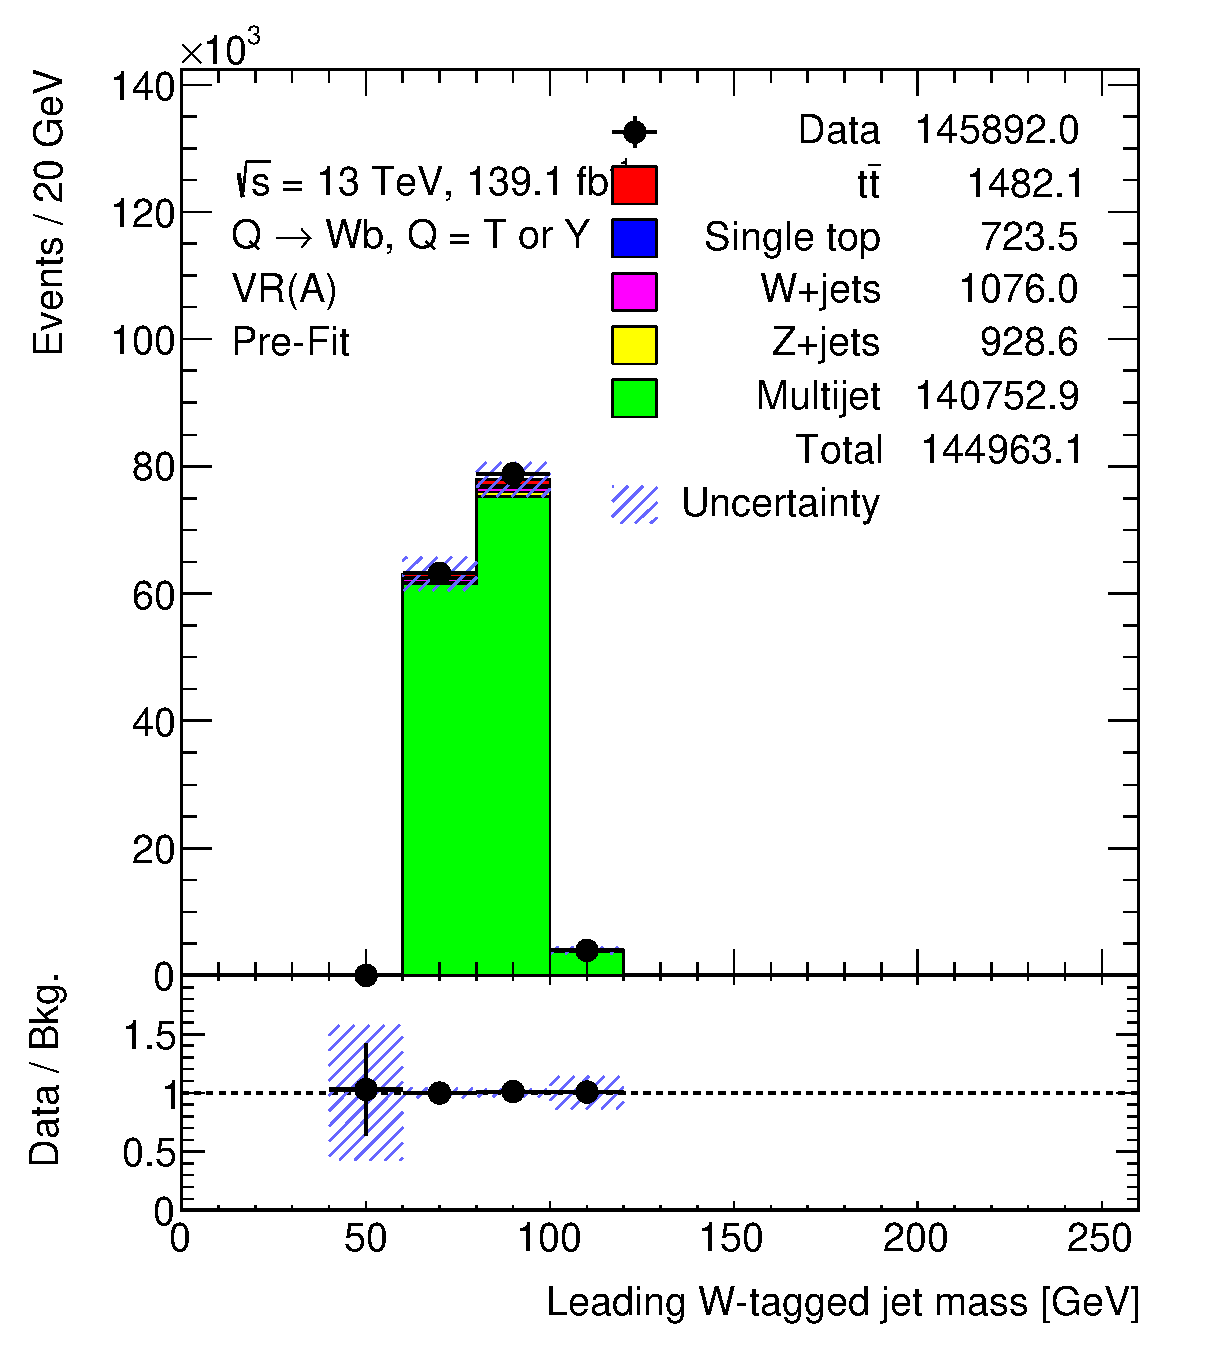
\includegraphics[width=\linewidth,height=\textheight,keepaspectratio]{VR_B_ljet_m.eps}
		\caption{}
		\label{fig:abcd:estimate:ljet_m}
	\end{subfigure}\hspace{0.6cm}
	\begin{subfigure}{.35\textwidth}
		\centering
		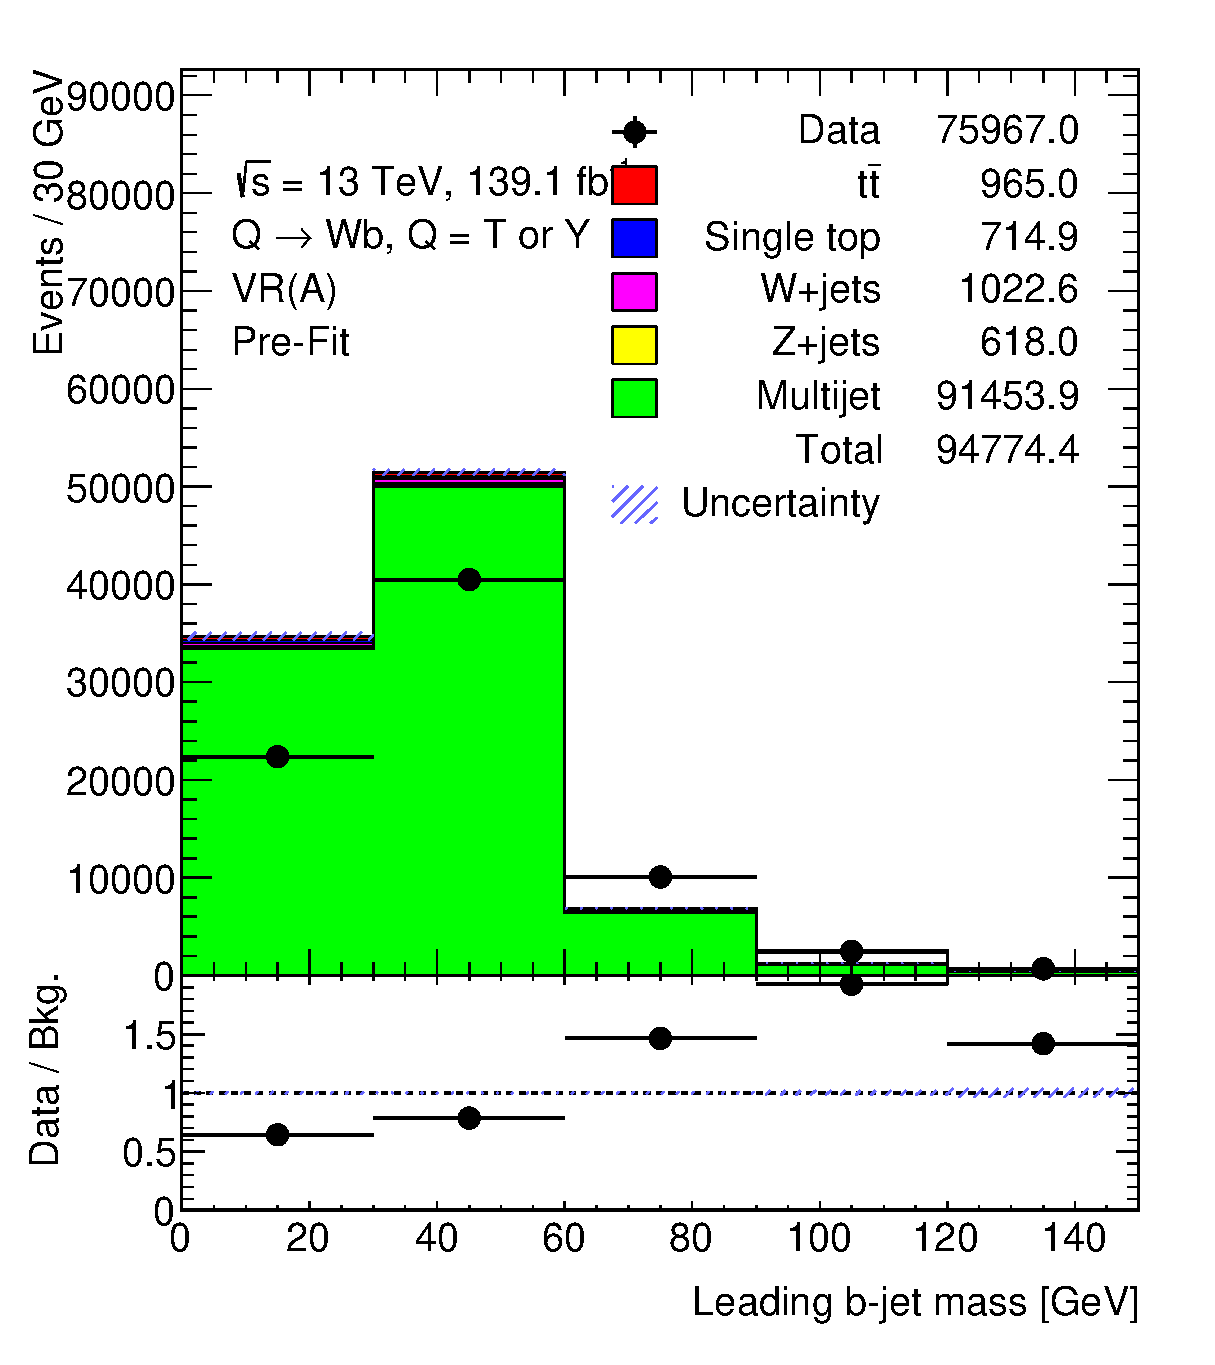
\includegraphics[width=\linewidth,height=\textheight,keepaspectratio]{VR_B_jet_m.eps}
		\caption{}
		\label{fig:abcd:estimate:jet_m}
	\end{subfigure}
	\caption{A data/bkg.\ comparison of kinematic and reconstructed variables in VR A where multijet background (in green) is estimated from the ABCD method and other backgrounds are from the MC simulation. The variables include (a) $p_{\text{T}}$ of $W$-tagged large-$R$ jet, (b) $p_{\text{T}}$ of leading $b$-tagged small-$R$ jet, (c) VLQ mass reconstructed from the kinematics of $W$-tagged large-$R$ jet and leading $b$-tagged small-$R$ jet, (d) $\eta$ distribution of $W$-tagged large-$R$ jet, (e) mass of $W$-tagged large-$R$ jet, and (f) mass of leading $b$-tagged small-$R$ jet.}
	\label{fig:abcd:estimate}
\end{figure}

%==============================================================================
\subsection{Need for correction}
\label{sec:abcd:estimate:need}
%==============================================================================
From the multijet estimate using the ABCD method shown in Fig.\ \ref{fig:abcd:estimate}, a general disagreement in data/bkg.\ can be seen. This is because one of the assumptions is not fulfulled. The choice of the variables in this thesis is in such a way to make sure there should be a minimal correlation which can be neglected. However, from the disagreement, it can be seen that there is a small amount of correlation in the two variables which needs to be taken into account. 

Moreover, the regions defined on the multiplicity of $b$-jets have different kinematics of the leading small-$R$ jet. This leading small-$R$ jet is further used to reconstruct the VLQ mass. The difference can be seen quite well from the distributions in the CRs shown in Appendix \ref{sec:app}. In that case, the ABCD relation given by Eqn.\ \ref{eqn:abcd:method} does not hold anymore and should be re-written as:

\begin{equation}
\frac{N_{\text{A}}}{N_{\text{B}}} \propto \frac{N_{\text{D}}}{N_{\text{C}}} \,,
\label{eqn:abcd:estimate:need}
\end{equation}
where $N_{\text{j}}$ is denoted as the number of background events in region j $\in$ \{A,B,C,D\}.

Also, the nature of this correction should be taken into account. Fig.\ \ref{fig:abcd:estimate:ljet_eta} shows that the correction should be implemented in such a way that a scale factor should be introduced. Then the distribution can be multiplied by this scale factor. In contrast, other distributions which are shown in Fig.\ \ref{fig:abcd:estimate} (a), (b), (c) and (f) say that this correction should be implemented for each bin separately in order to fix the shape of the distribution.


%==============================================================================
\section{Correction factor}
\label{sec:abcd:correctionfactor}
%==============================================================================
From the previous section, it has been seen that there is a need to introduce a correction factor to the ABCD equation. So, Eqn.\ \ref{eqn:abcd:estimate} can be re-written as :

\begin{equation}
N_{\text{A}}^{\text{Est.\ multijet}}[i] = \R \times (N_{\text{B}}^{\text{Data}}[i]-N_{\text{B}}^{\text{Other bkg}}[i]) \times \frac{(N_{\text{D}}^{\text{Data}}[i]-N_{\text{D}}^{\text{Other bkg}}[i])}{(N_{\text{C}}^{\text{Data}}[i]-N_{\text{C}}^{\text{Other bkg}}[i])} \,,
\label{eqn:abcd:correctionfactor}
\end{equation}
where \R is a correction factor which is calculated from multijet MC samples. It can be calculated in two different ways depending upon the nature of the correction.

\begin{itemize}
	\item \textbf{Normalisation method:} \R is calculated to compensate for the difference in the normalisation of the estimated multijet and the data. It is calculated by the expression given below:
	
	\begin{equation}
		\R = \frac{\N{A}{multijet MC}}{\N{B}{multijet MC}} \times \frac{\N{C}{multijet MC}}{\N{D}{multijet MC}} \,,
	\end{equation}
	where \N{j}{multijet MC} is the number of multijet events from MC sample in region $j\in\{A, B, C, D\}$, which can be calculated by taking the integral of the distribution. So, in the end, \R is a number which can be used in Eqn.\ \ref{eqn:abcd:correctionfactor} to scale the estimated multijet.
	
	\item \textbf{Shape method:} \R is calculated to fix the shape of the distributions by calculating it bin-by-bin. A corresponding expression can be written as:
	
	\begin{equation}
	\R[i] = \frac{\N{A}{multijet MC}[i]}{\N{B}{multijet MC}[i]} \times \frac{\N{C}{multijet MC}[i]}{\N{D}{multijet MC}[i]} \,,
	\end{equation}
	where $[i]$ shows that the calculation is performed for each bin separately within a distribution ($i=$ bin). So, it leads to a separate \R$[i]$ distribution for each kinematic variables, which can further be used to correct the estimated multijet.
\end{itemize}

The difference between the two methods is that \R from the normalisation method would be a number which is independent of distribution and can be used to scale the estimated multijet of all the kinematic distributions whereas \R$[i]$ from the shape method is a distribution dependent correction factor and would be different for every kinematic distribution.

The correction factor is calculated from both the methods. A value for the correction factor comes out to be \R = 1.26 in the case of normalisation method, which is used to scale the estimated multijet from the ABCD method in all the six distributions shown in Fig.\ \ref{fig:abcd:estimate}. Similarly, \R$[i]$ from shape method is also evaluated, and six different distributions are obtained, which are further multiplied with their respective six distributions to get the estimated multijet. 

Fig.\ \ref{fig:abcd:correctionfactor:ljet_pt} shows the \pt distribution of $W$-tagged large-$R$ jet when \R is calculated from both the methods. The estimated multijet agrees well with the data when \R is calculated using the shape method as shown in Fig.\ \ref{fig:abcd:correctionfactor:bin:ljet_pt}. A significant difference can be seen in the \pt distribution of leading $b$-tagged jet in Fig.\ \ref{fig:abcd:correctionfactor:jet_pt} where \R has compensated well at low \pt when it is calculated by the shape method. A similar kind of effect can also be seen at the first bin of VLQ mass distribution in Fig.\ \ref{fig:abcd:correctionfactor:VLQM}. On the other hand, $\eta$ distribution of $W$-tagged large-$R$ in Fig.\ \ref{fig:abcd:correctionfactor:ljet_eta} shows that there is not much difference between the two methods. This is because the $\eta$ distribution is a uniform distribution and scaling the distribution or applying correction bin-by-bin does create a significant difference. However, looking at the event yields of multijet in the two distributions, it can be inferred that calculation from normalisation method shows better results than the shape method. The priority is bin-by-bin agreement of the data and estimated multijet in all the distributions. The error shown in the plots is all statistical uncertainty which is discussed in detail in the next chapter.


\begin{figure}[hbt!]
	\centering
	\begin{subfigure}{.35\textwidth}
		\centering
		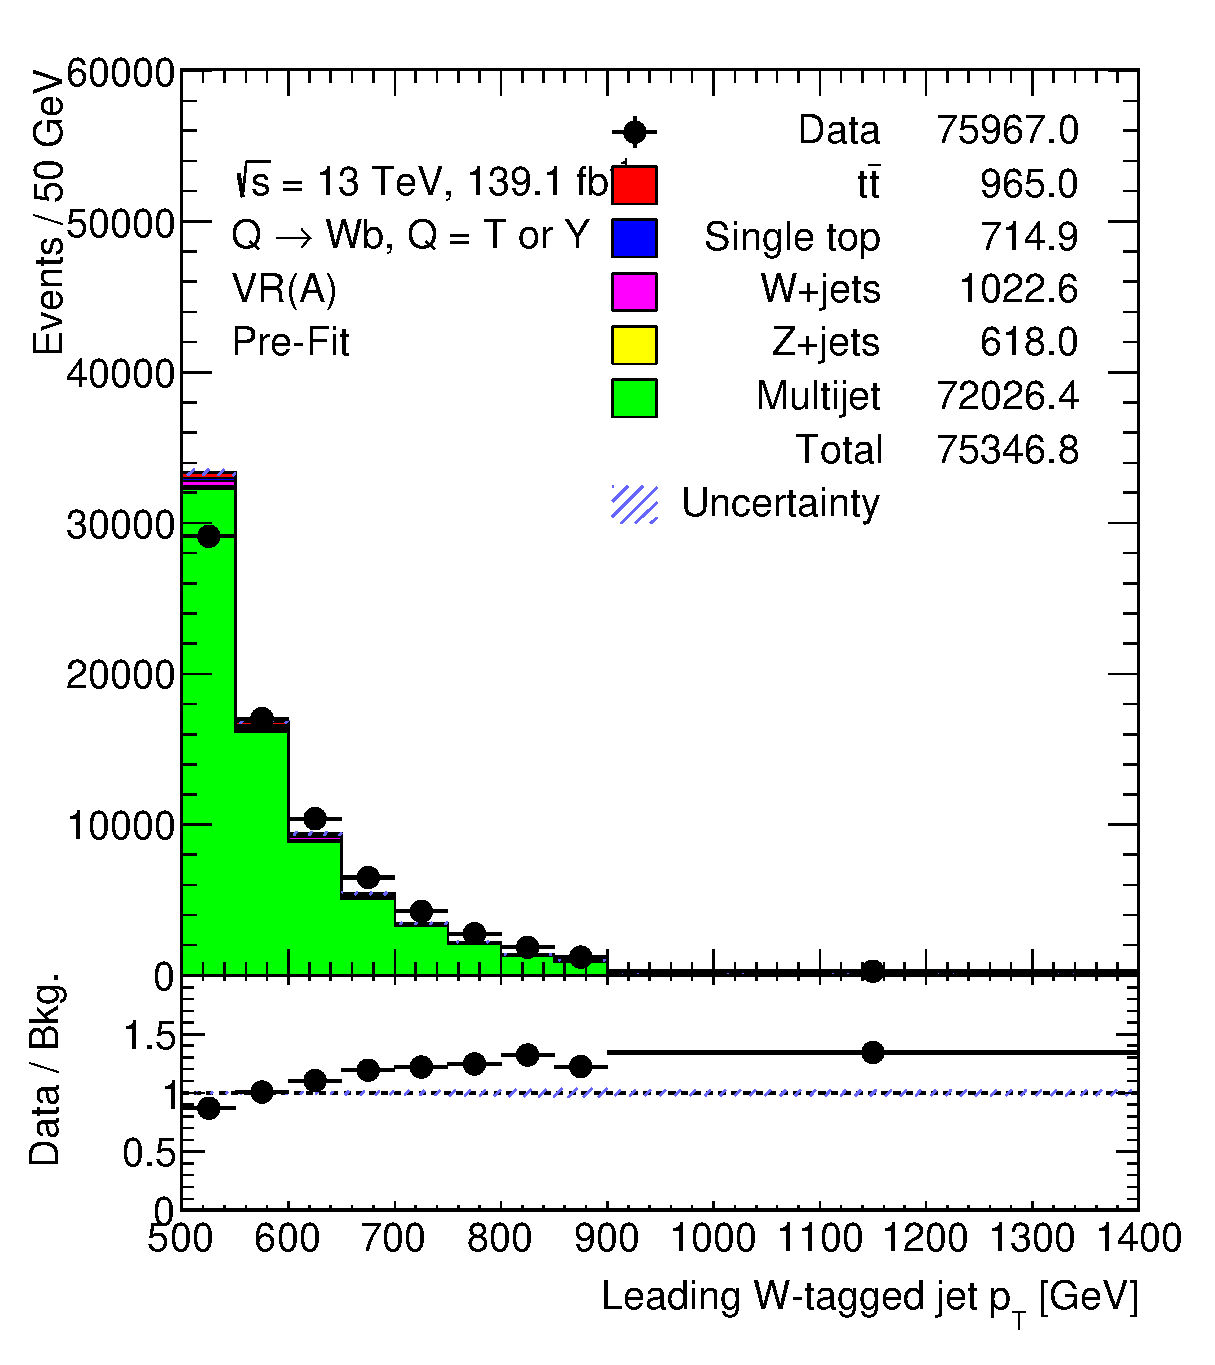
\includegraphics[width=\linewidth,height=\textheight,keepaspectratio]{figs/chapter5/prefitintegral/VR_B_ljet_pt.eps}
		\caption{}
		\label{fig:abcd:correctionfactor:integral:ljet_pt}
	\end{subfigure}\hspace{0.6cm}
	\begin{subfigure}{.35\textwidth}
		\centering
		\includegraphics[width=\linewidth,height=\textheight,keepaspectratio]{figs/chapter5/prefitbinbybin/VR_B_ljet_pt.eps}
		\caption{}
		\label{fig:abcd:correctionfactor:bin:ljet_pt}
	\end{subfigure}
	\caption{Comparison between the estimated multijet when \R is calculated by (a) normalisation method and (b) shape method in the \pt distribution of $W$-tagged large-$R$ jet.}
	\label{fig:abcd:correctionfactor:ljet_pt}
\end{figure}


\begin{figure}[hbt!]
	\centering
	\begin{subfigure}{.35\textwidth}
		\centering
		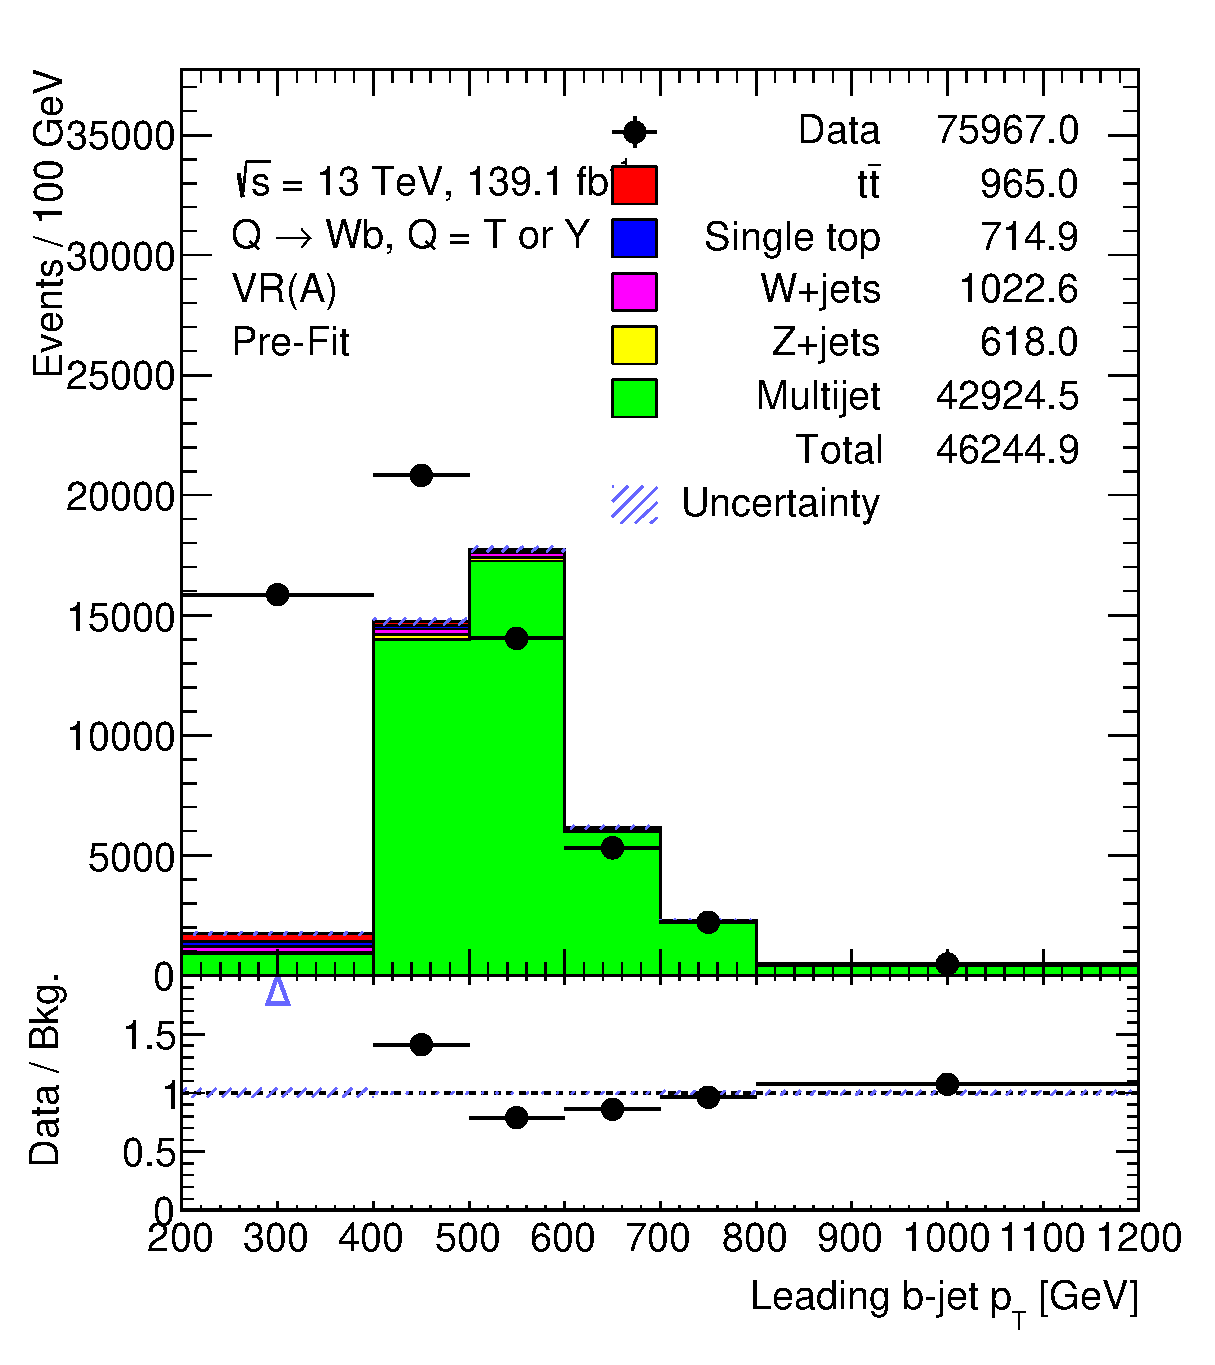
\includegraphics[width=\linewidth,height=\textheight,keepaspectratio]{figs/chapter5/prefitintegral/VR_B_jet_pt.eps}
		\caption{}
		\label{fig:abcd:correctionfactor:integral:jet_pt}
	\end{subfigure}\hspace{0.6cm}
	\begin{subfigure}{.35\textwidth}
		\centering
		\includegraphics[width=\linewidth,height=\textheight,keepaspectratio]{figs/chapter5/prefitbinbybin/VR_B_jet_pt.eps}
		\caption{}
		\label{fig:abcd:correctionfactor:bin:jet_pt}
	\end{subfigure}
	\caption{Comparison between the estimated multijet when \R is calculated by (a) normalisation method and (b) shape method in the \pt distribution of leading $b$-tagged jet.}
	\label{fig:abcd:correctionfactor:jet_pt}
\end{figure}


\begin{figure}[hbt!]
	\centering
	\begin{subfigure}{.35\textwidth}
		\centering
		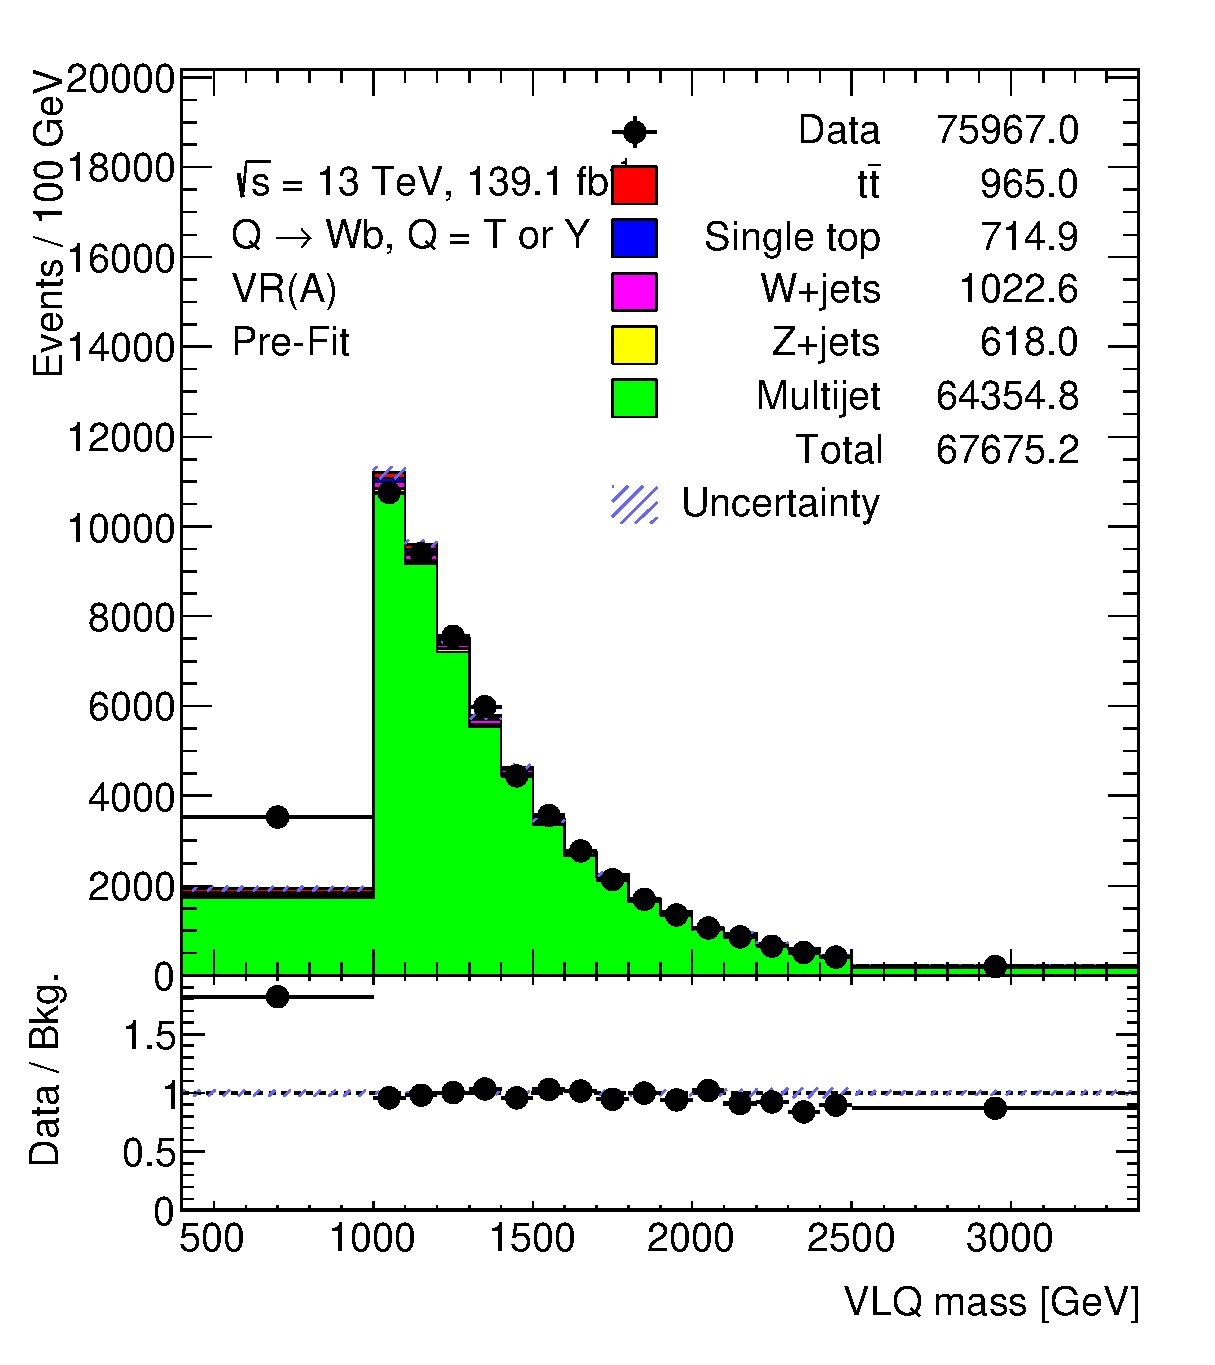
\includegraphics[width=\linewidth,height=\textheight,keepaspectratio]{figs/chapter5/prefitintegral/VR_B_VLQM.eps}
		\caption{}
		\label{fig:abcd:correctionfactor:integral:VLQM}
	\end{subfigure}\hspace{0.6cm}
	\begin{subfigure}{.35\textwidth}
		\centering
		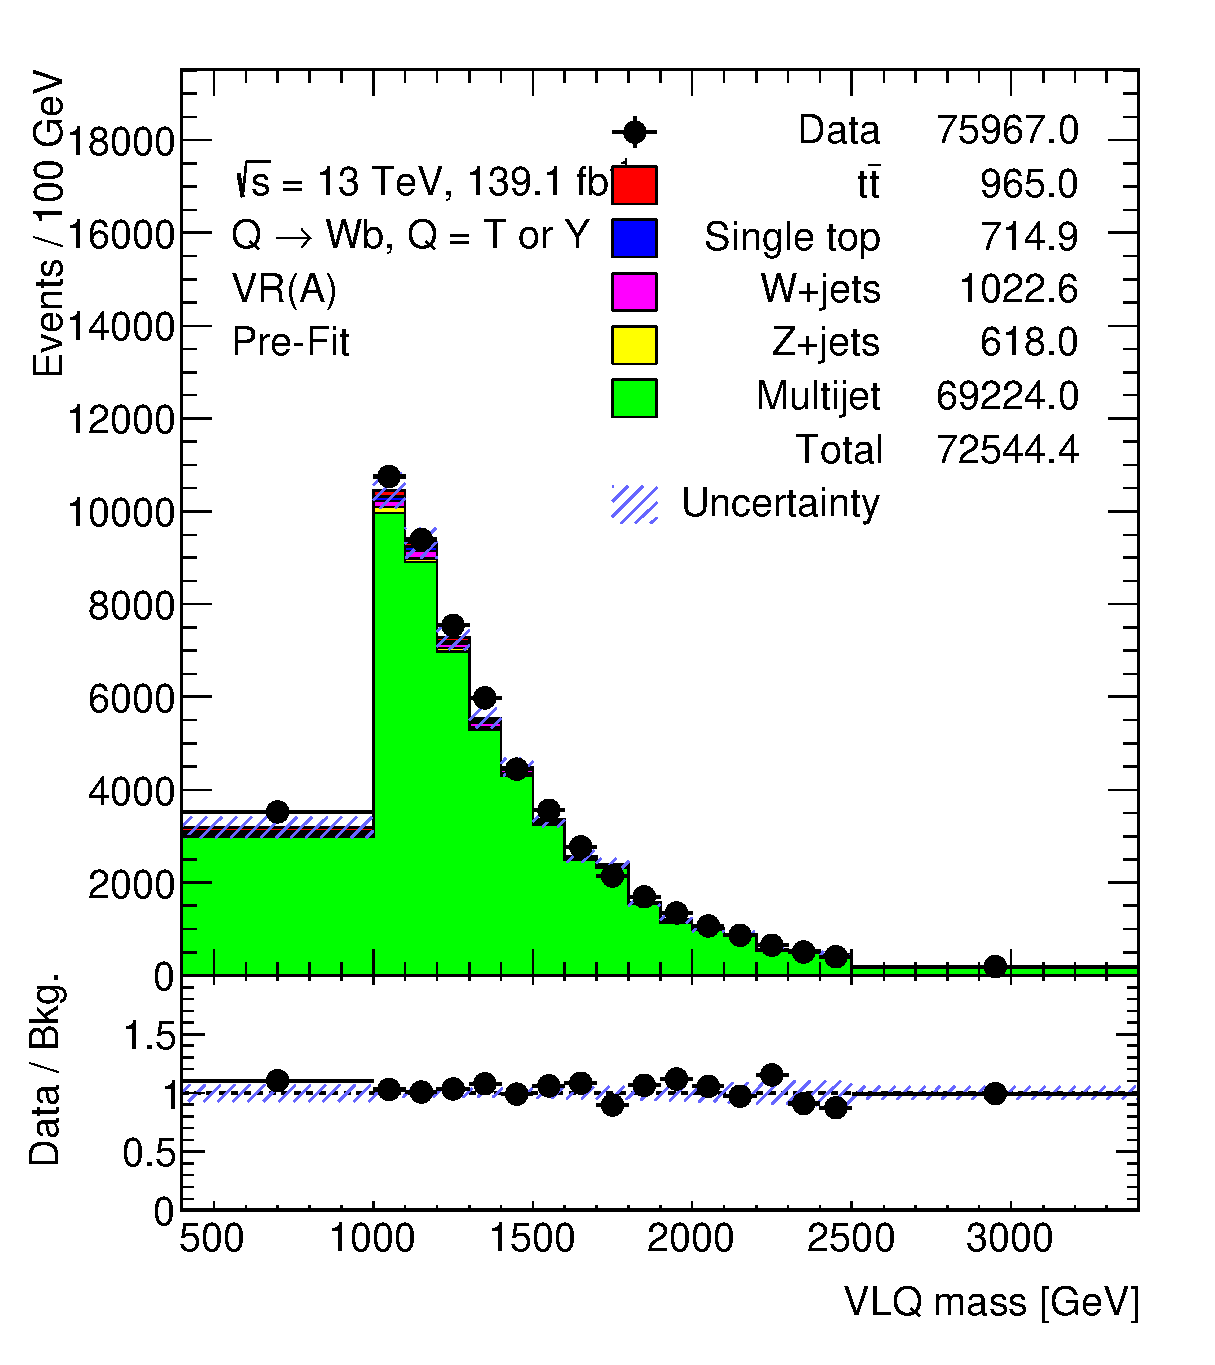
\includegraphics[width=\linewidth,height=\textheight,keepaspectratio]{figs/chapter5/prefitbinbybin/VR_B_VLQM.eps}
		\caption{}
		\label{fig:abcd:correctionfactor:bin:VLQM}
	\end{subfigure}
	\caption{Comparison between the estimated multijet when \R is calculated by (a) normalisation method and (b) shape method in the VLQ mass distribution.}
	\label{fig:abcd:correctionfactor:VLQM}
\end{figure}


\begin{figure}[hbt!]
	\centering
	\begin{subfigure}{.35\textwidth}
		\centering
		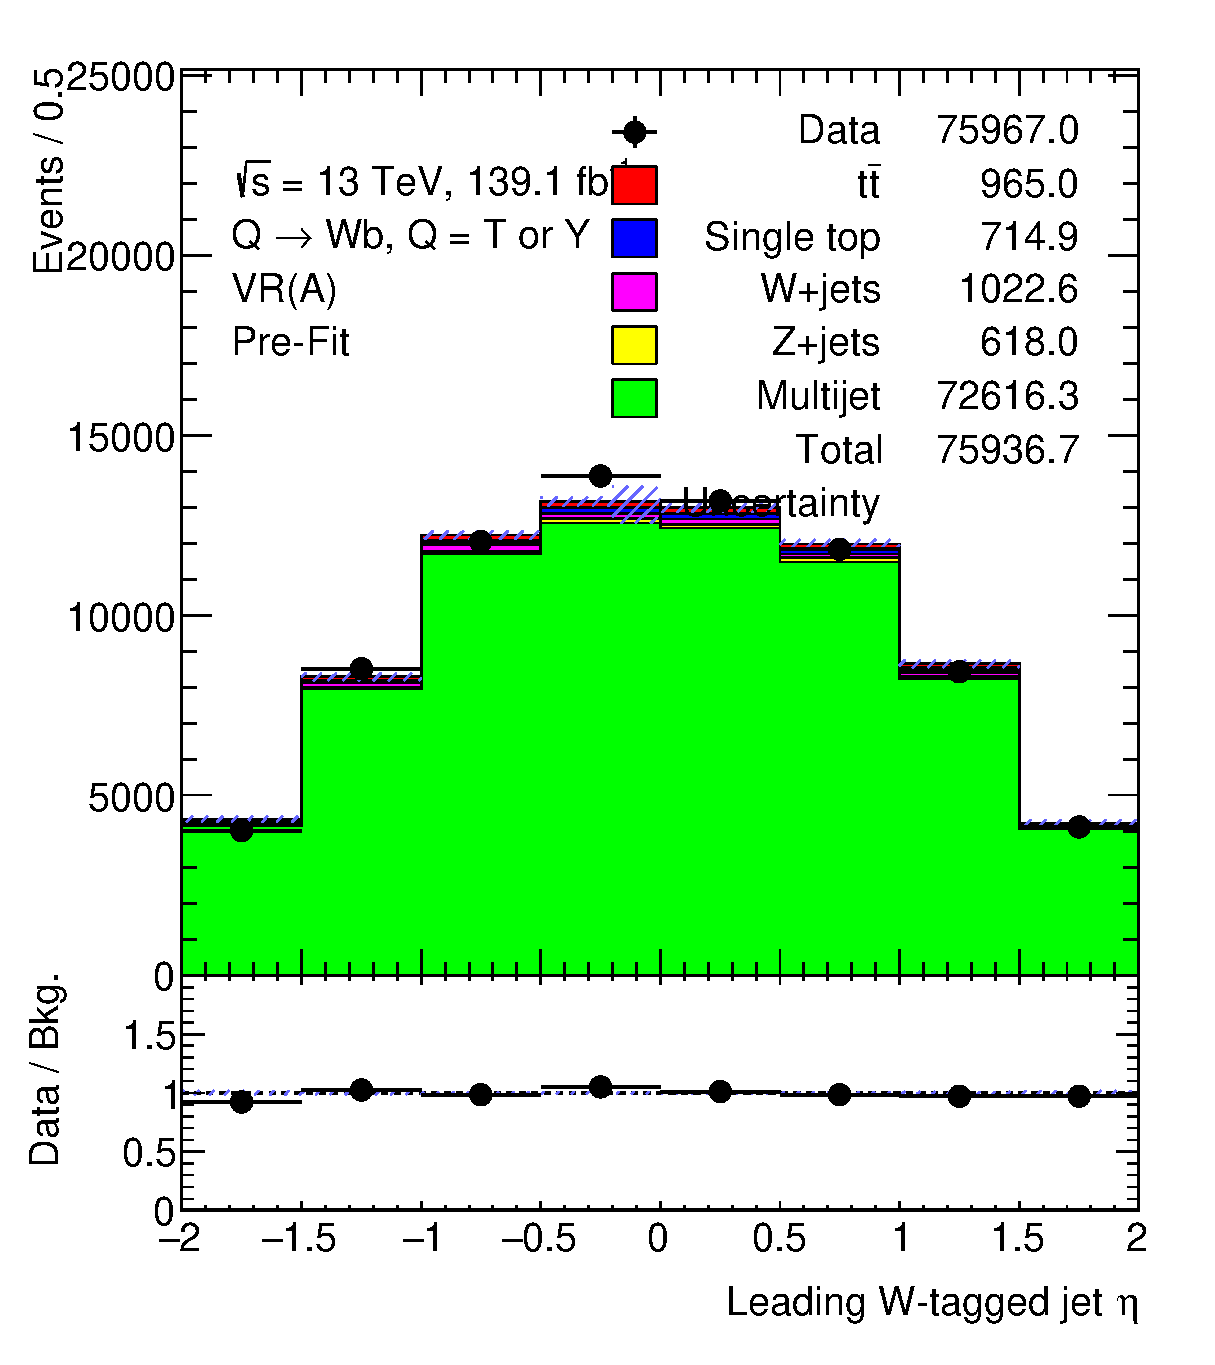
\includegraphics[width=\linewidth,height=\textheight,keepaspectratio]{figs/chapter5/prefitintegral/VR_B_ljet_eta.eps}
		\caption{}
		\label{fig:abcd:correctionfactor:integral:ljet_eta}
	\end{subfigure}\hspace{0.6cm}
	\begin{subfigure}{.35\textwidth}
		\centering
		\includegraphics[width=\linewidth,height=\textheight,keepaspectratio]{figs/chapter5/prefitbinbybin/VR_B_ljet_eta.eps}
		\caption{}
		\label{fig:abcd:correctionfactor:bin:ljet_eta}
	\end{subfigure}
	\caption{Comparison between the estimated multijet when \R is calculated by (a) normalisation method and (b) shape method in the $\eta$ distribution of $W$-tagged large-$R$ jet.}
	\label{fig:abcd:correctionfactor:ljet_eta}
\end{figure}

\clearpage
%==============================================================================
\section{Further improvement}
\label{sec:abcd:furtherimprovement}
%==============================================================================
After applying the \R, the multijet estimate shows a good agreement with the data. However, there is still a room for improvement. At preselection, it has been observed that the data/MC mismodelling is flat in \pt and VLQ mass, as shown in Fig.\ \ref{fig:analysisstrategy:eventselection:preselection}. Also, in the hadronic channel, one cannot trust the multijet MC  because of the mismodelling. But the correction factor in the previous section was calculated from these mismodelled multijet MC. So, in order to make the estimate purely data-driven process, a likelihood fit is performed to fit multijet MC to the data. So, in this section, the process of fitting the multijet MC to data is discussed along with how it has improved the estimation.
%==============================================================================
\subsection{Fitting}
\label{sec:abcd:furtherimprovement:fitting}
%==============================================================================
The aim is to determine the correction factor from the data. The task can be encoded into a statistical model where multijet behaves according to the observed data which can be represented by a parameter. A maximum likelihood fit~\cite{likelihood} of the model to data is used to obtain the parameter estimate. Then, the multijet MC is scaled with this parameter estimate. The whole process is implemented by the maximum likelihood method.

\paragraph{Maximum likelihood method} 
Let us consider the Poisson distribution that describes the observed event yields in an experiment.~\cite{thesis:rui} 
\begin{equation}
	\mathcal{P}(n|\lambda) = \lambda^{n} \frac{e^{-\lambda}}{n!} \,,
\end{equation}
where $n$ is denoted as the observed event yields and $\lambda$ is represented as the expected event yields.

Let us suppose an observable $x$ follows a distribution $f(x)$, the likelihood of the parameter $\lambda$ can be expressed as:
\begin{equation}
\mathcal{L}(\lambda) = \mathcal{P}(n|\lambda) \prod_{\text{event}}^{n} f(x) \,.
\end{equation}
The function $f(x)$ is usually described by histograms, where the observable $x$ is binned to discrete values. The event yields in each bin are Poisson distributed, making the likelihood a product of multiple Poisson distributions. It is also known as the \textit{binned likelihood} and can be written as:

\begin{equation}
\mathcal{L}(\lambda_{\text{b}}) = \prod_{\text{b$\in$bins}}^{} \mathcal{P}(n_{\text{b}}|\lambda_{\text{b}}) \,.
\end{equation}

Likelihood is multiplicative, so when it is performed for more than one region together, such as various control regions together, then it can be written as:

\begin{equation}
\mathcal{L}(\lambda_{\text{b,r}}) = \prod_{\text{r$\in$regions}}^{}\prod_{\text{b$\in$bins}}^{} \mathcal{P}(n_{\text{b,r}}|\lambda_{\text{b,r}}) \,,
\end{equation}
where $n_{\text{b,r}}$ and $\lambda_{\text{b,r}}$ are denoted as the number of observed events and the true events in a given bin of a given region respectively.

In most cases, log-likelihood functions are used because it converts the product of likelihoods into a simple summation which can be written as:

\begin{equation}
\text{ln }\mathcal{L}(\lambda_{\text{b,r}}) = \sum_{\text{r$\in$regions}}^{}\sum_{\text{b$\in$bins}}^{} \text{ln }\mathcal{P}(n_{\text{b,r}}|\lambda_{\text{b,r}}) \,.
\label{eqn:abcd:furtherimprovement:fitting}
\end{equation}
Now, the expression can be maximised to give an estimate of $\lambda_{\text{b,r}}$ denoted as $\hat{\lambda}_{\text{b,r}}$.

\begin{equation}
	\frac{\partial\text{ln } \mathcal{L}(\lambda_{\text{b,r}})}{\partial \lambda_{\text{b,r}}} \bigg|_{\lambda_{\text{b,r}}=\hat{\lambda}_{\text{b,r}}} = 0 \,.
\end{equation}

Sometimes it is challenging to perform this calculation analytically. In such cases, a set of computer programs which are based on numerical methods are generally preferred. In this thesis, a package called \textsc{TrexFitter}, which is based on \textsc{RooStats}~\cite{roostats} is used to perform the likelihood fit.
%==============================================================================
\subsection{Implementation on the multijet MC}
\label{sec:abcd:furtherimprovement:scaledcorr}
%==============================================================================
The maximumm likelihood method is performed to fit multijet MC to the data. It can only be applied in VR A since the data is blinded in SR A1. So, region A, B, C and D are taken into account. The fit is performed in region A and B together and region C and D together instead of fitting it individually because the regions should be correlated, and the multijet MC should be scaled by the same amount in the two regions where their normalisation is completely correlated.

In Eqn.\ \ref{eqn:abcd:furtherimprovement:fitting}, the expected event yield is predicted by the MC samples which contain both signal and background events. So, $\lambda_{\text{b,r}}$ can be expressed as:
\begin{equation}
	\lambda_{\text{b,r}} = \mu\lambda_{\text{b,r}}^{\text{sig. MC}} + (\lambda_{\text{b,r}}^{\text{other bkg. MC}} + \lambda_{\text{b,r}}^{\text{multijet MC}} ) \,,
\end{equation}
where $\mu$ is signal strength. The fit is performed as a background only fit, i.e.\ $\mu = 0$, while keeping the normalisation of the multijet as a free parameter. The normalisation of the other backgrounds is kept constant.

So, the log-likelihood function for region A and B together can be written as: 
\begin{equation}
\text{ln }\mathcal{L}(\lambda_{\text{b,r}}) = \sum_{\text{r$\in$\{A,B\}}}^{}\sum_{\text{b$\in$bins}}^{} \text{ln }\mathcal{P}(n_{\text{b,r}}|\lambda_{\text{b,r}}) \,.
\end{equation}
Similarly, the log-likelihood function for region C and D together can be written as: 
\begin{equation}
\text{ln }\mathcal{L}(\lambda_{\text{b,r}}) = \sum_{\text{r$\in$\{C,D\}}}^{}\sum_{\text{b$\in$bins}}^{} \text{ln }\mathcal{P}(n_{\text{b,r}}|\lambda_{\text{b,r}}) \,.
\end{equation}
These likelihood functions are maximised to get an estimate of $\hat{\lambda}_{\text{b,r}}$. It is performed for all the six variables separately to get six distributions where the multijet MC are fitted to the data, so we call it scaled multijet MC. The distribution for some kinematic variables for both multijet MC and scaled multijet MC in all the four regions A, B, C and D are shown in Appendix \ref{sec:app2}.


%==============================================================================
\subsection{Calculation of \R from the scaled multijet MC}
\label{sec:abcd:furtherimprovement:rcorr}
%==============================================================================
Now, \R is calculated from the scaled multijet MC (as discussed in the previous section) again by using two methods. It is calculated for each kinematic distribution separately.

\begin{itemize}
	\item \textbf{Normalisation method:} it is calculated by the expression given below:
	
	\begin{equation}
	\R = \frac{\N{A}{scaled multijet MC}}{\N{B}{scaled multijet MC}} \times \frac{\N{C}{scaled multijet MC}}{\N{D}{scaled multijet MC}} \,,
	\end{equation}
	where \N{j}{scaled multijet MC} is the number of events from the scaled multijet MC in region $j\in\{A, B, C, D\}$, which can be calculated by taking the integral of the distribution. So, in the end, \R is a number which can be used in Eqn.\ \ref{eqn:abcd:correctionfactor} to scale the estimated multijet. Note that now this number is not same for all the kinematic distributions because the multijet MC in each kinematic distribution is scaled differently in the scaled multijet MC distributions. Table \ref{table:abcd:furtherimprovement:rcorr} shows the value of \R for all the six distributions.
	
	\begin{table}[hbt!]
		\centering
		\begin{tabular}{c|c|c|c|c|c|c} 
			\toprule
			Kinematic  & \multicolumn{3}{c}{$W$-tagged jet} \vline & \multicolumn{2}{c}{leading $b$-tagged jet} \vline & VLQ mass\\ \cline{2-6}
			distribution & \pt & mass & $\eta$ & \pt & mass & \\ 
			\midrule
			\R & \num{1.31} & \num{1.32} & \num{1.33} & \num{1.34} & \num{1.33} & \num{1.33} \\
			\bottomrule
		\end{tabular}
		\caption{Value of \R for all the six kinematic distributions calculated from the scaled multijet MC by using normalisation method.}
		\label{table:abcd:furtherimprovement:rcorr}
	\end{table}
	
	\item \textbf{Shape method:} a corresponding expression can also be written as:
	\begin{equation}
	\R[i] = \frac{\N{A}{scaled multijet MC}[i]}{\N{B}{scaled multijet MC}[i]} \times \frac{\N{C}{scaled multijet MC}[i]}{\N{D}{scaled multijet MC}[i]} \,,
	\end{equation}
	where $[i]$ shows that the calculation is performed for each bin separately within a distribution ($i=$ bin). So, it leads to a separate \R$[i]$ distribution for each kinematic distribution, which can further be used to correct the estimated multijet in Eqn.\ \ref{eqn:abcd:correctionfactor}.
\end{itemize}


Summing up, in this thesis, \R is calculated from four different methods:
\begin{enumerate}
	\item From multijet MC by using normalisation method. (described in section \ref{sec:abcd:correctionfactor})
	\item From multijet MC by using shape method. (described in section \ref{sec:abcd:correctionfactor})
	\item From scaled multijet MC by using normalisation method.
	\item From scaled multijet MC by using shape method.
\end{enumerate}

A data/bkg.\ comparison plot is shown in Fig.\ \ref{fig:abcd:furtherimprovement:scaledcorr:VLQM}, where the estimated multijet is shown in VLQ mass distribution when \R is calculated from all the four methods. It can be observed that \R calculated from normalisation method does not produce any significant difference when it is calculated from either multijet MC or scaled multijet MC. However, better results in the estimate can be seen from the shape method, especially in the event yields of the estimated multijet. A detailed event yields of the estimated multijet when \R is calculated from all the four methods are shown in Table \ref{table:abcd:furtherimprovement:scaledcorr}. 

So, in general Fig.\ \ref{fig:abcd:furtherimprovement:scaledcorr:postfit:bin:VLQM} shows the best estimate of multijet background where \R is calculated from the scaled multijet MC by using shape method. The other distributions are also shown in Fig.\ \ref{fig:abcd:furtherimprovement:scaledcorr} to confirm that the method works efficiently in all the other distributions as well. So, this multijet estimate is regarded as the final estimate.

\begin{table}[hbt!]
	\centering
	\begin{tabular}{c|c|c|c|c} 
		\toprule
		Sample & \multicolumn{2}{c}{Multijet MC} \vline & \multicolumn{2}{c}{Scaled multijet MC} \\ \cline{2-5} 
		 & Normalisation & Shape & Normalisation & Shape \\ 
		\midrule
		Data & 75967 & 75967 & 75967 & 75967 \\
		Other bkg. & $\num{3320}\pm\num{95}$ & $\num{3320}\pm\num{95}$ & $\num{3320}\pm\num{95}$ & $\num{3320}\pm\num{95}$ \\
		Est. multijet & $\num{72616}\pm\num{304}$ & $\num{69398}\pm\num{914}$ & $\num{71901}\pm\num{301}$ & $\num{72613}\pm\num{305}$ \\
		\midrule
		Total bkg. & $\num{75936}\pm\num{319}$ & $\num{72718}\pm\num{919}$ & $\num{75221}\pm\num{316}$ & $\num{75933}\pm\num{319}$ \\
		\bottomrule
	\end{tabular}
	\caption{Event yields of the estimated multijet background in VR A from the ABCD method when \R is calculated from all the four methods. The errors shown here are from statistical uncertainty.}
	\label{table:abcd:furtherimprovement:scaledcorr}
\end{table}

\begin{figure}[hbt!]
	\centering
	\begin{subfigure}{.35\textwidth}
		\centering
		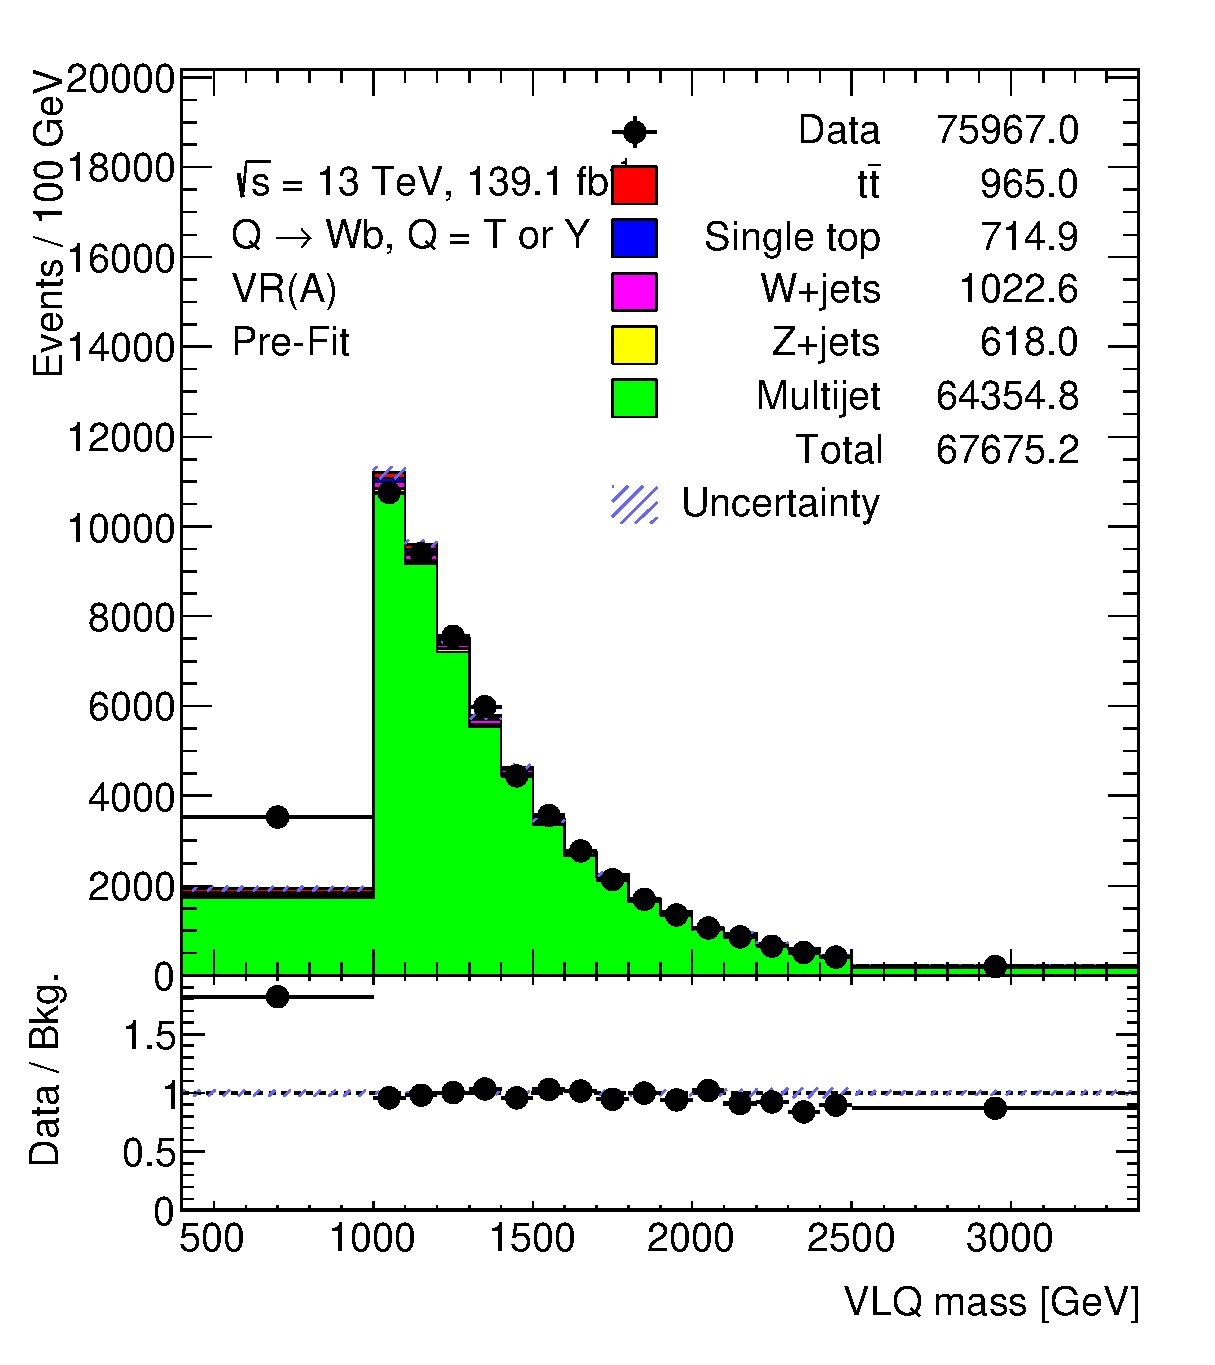
\includegraphics[width=\linewidth,height=\textheight,keepaspectratio]{figs/chapter5/prefitintegral/VR_B_VLQM.eps}
		\caption{}
		\label{fig:abcd:furtherimprovement:scaledcorr:prefit:integral:VLQM}
	\end{subfigure}\hspace{0.6cm}
	\begin{subfigure}{.35\textwidth}
		\centering
		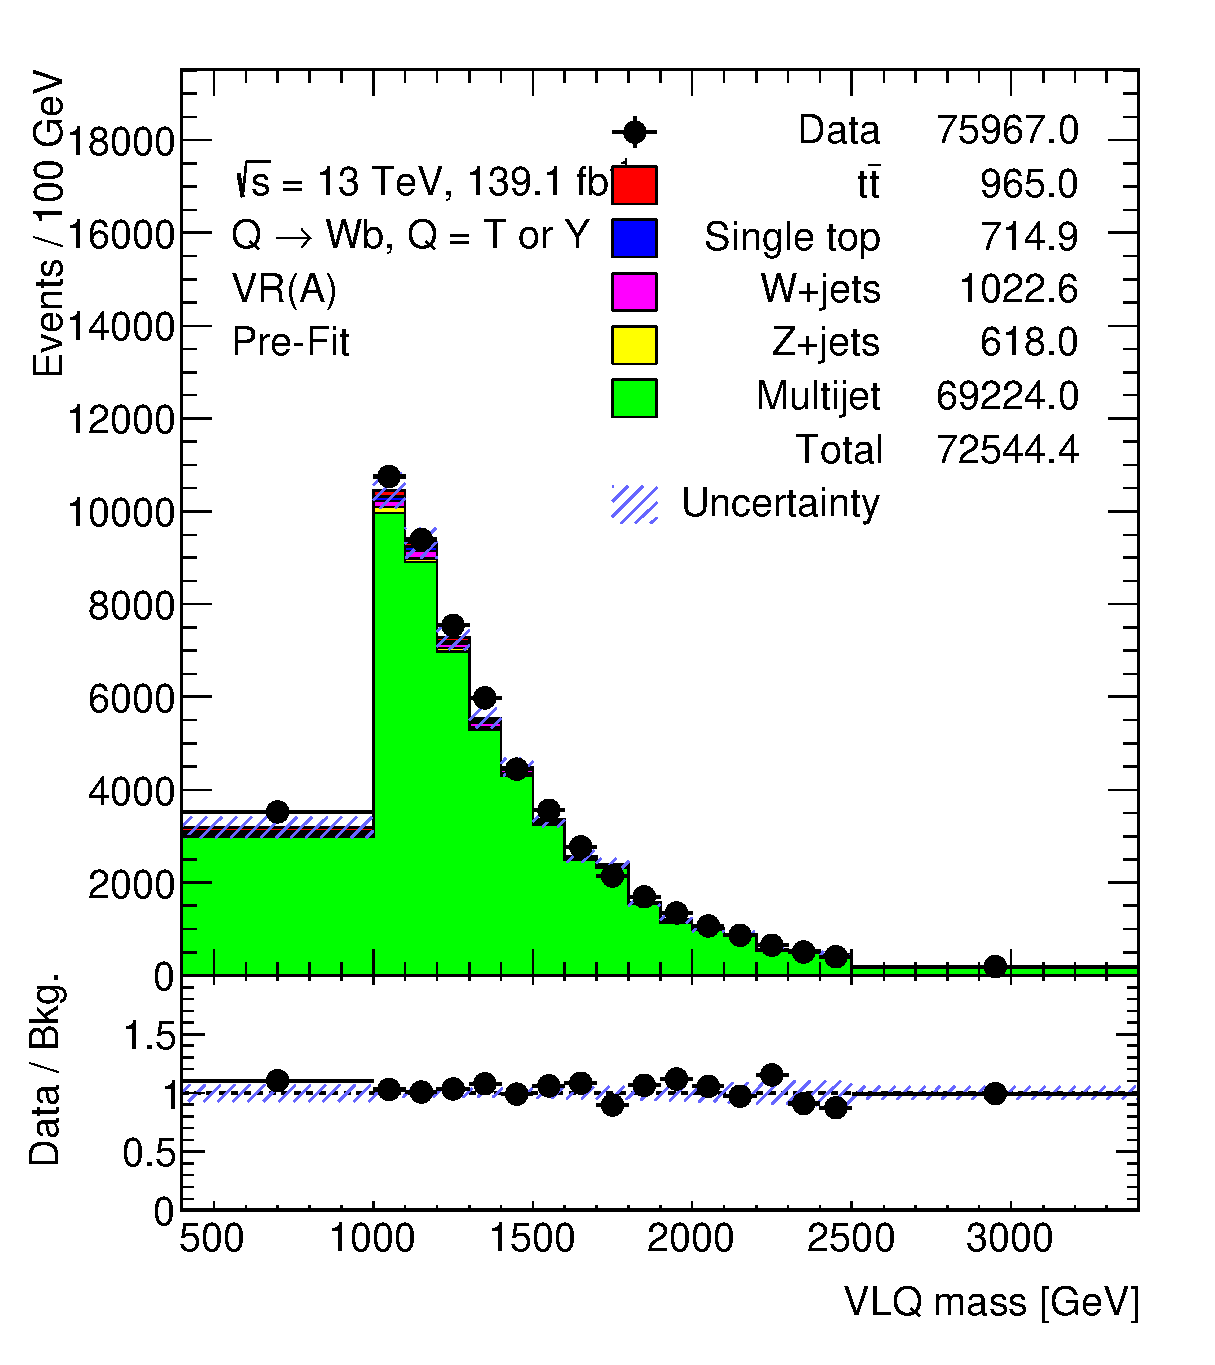
\includegraphics[width=\linewidth,height=\textheight,keepaspectratio]{figs/chapter5/prefitbinbybin/VR_B_VLQM.eps}
		\caption{}
		\label{fig:abcd:furtherimprovement:scaledcorr:prefit:bin:VLQM}
	\end{subfigure}
	\begin{subfigure}{.35\textwidth}
		\centering
		\includegraphics[width=\linewidth,height=\textheight,keepaspectratio]{figs/chapter5/postfitintegral/VR_B_VLQM.eps}
		\caption{}
		\label{fig:abcd:furtherimprovement:scaledcorr:postfit:integral:VLQM}
	\end{subfigure}\hspace{0.6cm}
	\begin{subfigure}{.35\textwidth}
		\centering
		\includegraphics[width=\linewidth,height=\textheight,keepaspectratio]{figs/chapter5/postfitbinbybin/VR_B_VLQM.eps}
		\caption{}
		\label{fig:abcd:furtherimprovement:scaledcorr:postfit:bin:VLQM}
	\end{subfigure}
	\caption{VLQ mass distribution where multijet background is estimated when \R is calculated from the multijet MC by using (a) normalisation method and (b) shape method, and from the scaled multijet MC by (c) normalisation method and (d) shape method.}
	\label{fig:abcd:furtherimprovement:scaledcorr:VLQM}
\end{figure}


\begin{figure}[hbt!]
	\centering
	\graphicspath{{figs/chapter5/postfitbinbybin/}}
	\begin{subfigure}{.35\textwidth}
		\centering
		\includegraphics[width=\linewidth,height=\textheight,keepaspectratio]{VR_B_ljet_pt.eps}
		\caption{}
		\label{fig:abcd:furtherimprovement:scaledcorr:ljet_pt}
	\end{subfigure}\hspace{0.6cm}
	\begin{subfigure}{.35\textwidth}
		\centering
		\includegraphics[width=\linewidth,height=\textheight,keepaspectratio]{VR_B_jet_pt.eps}
		\caption{}
		\label{fig:abcd:furtherimprovement:scaledcorr:jet_pt}
	\end{subfigure}
	\begin{subfigure}{.35\textwidth}
		\centering
		\includegraphics[width=\linewidth,height=\textheight,keepaspectratio]{VR_B_ljet_eta.eps}
		\caption{}
		\label{fig:abcd:furtherimprovement:scaledcorr:ljet_eta}
	\end{subfigure}\hspace{0.6cm}
	\begin{subfigure}{.35\textwidth}
		\centering
		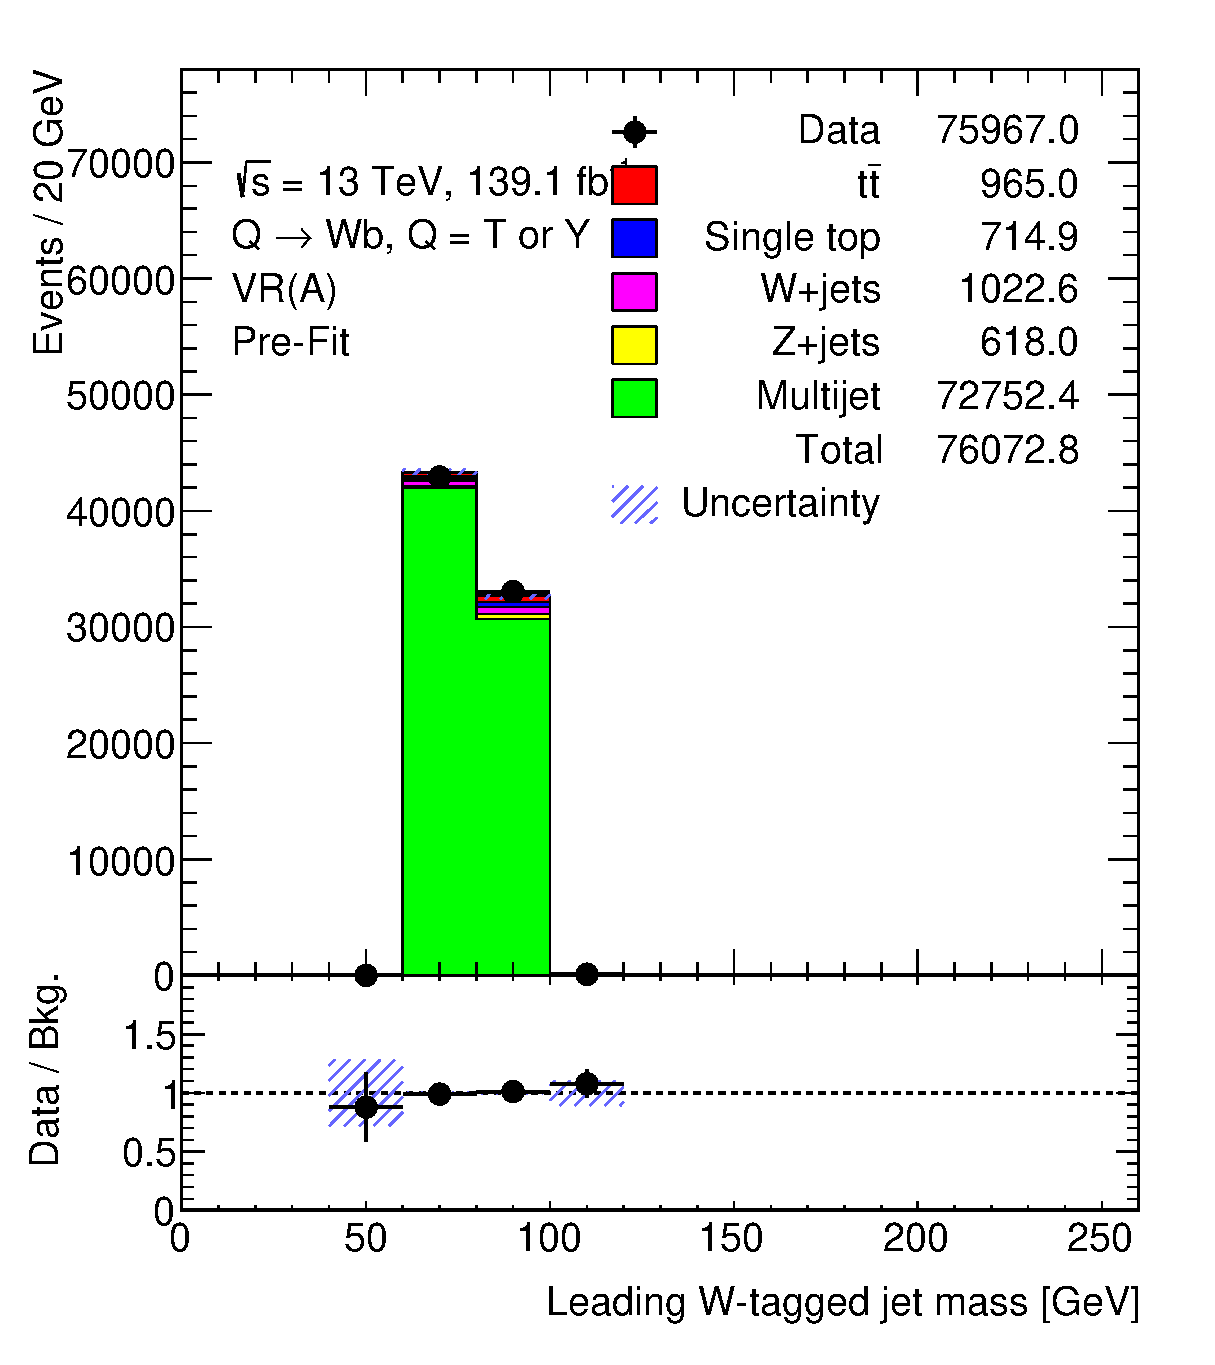
\includegraphics[width=\linewidth,height=\textheight,keepaspectratio]{VR_B_ljet_m.eps}
		\caption{}
		\label{fig:abcd:furtherimprovement:scaledcorr:ljet_m}
	\end{subfigure}
	\begin{subfigure}{.35\textwidth}
		\centering
		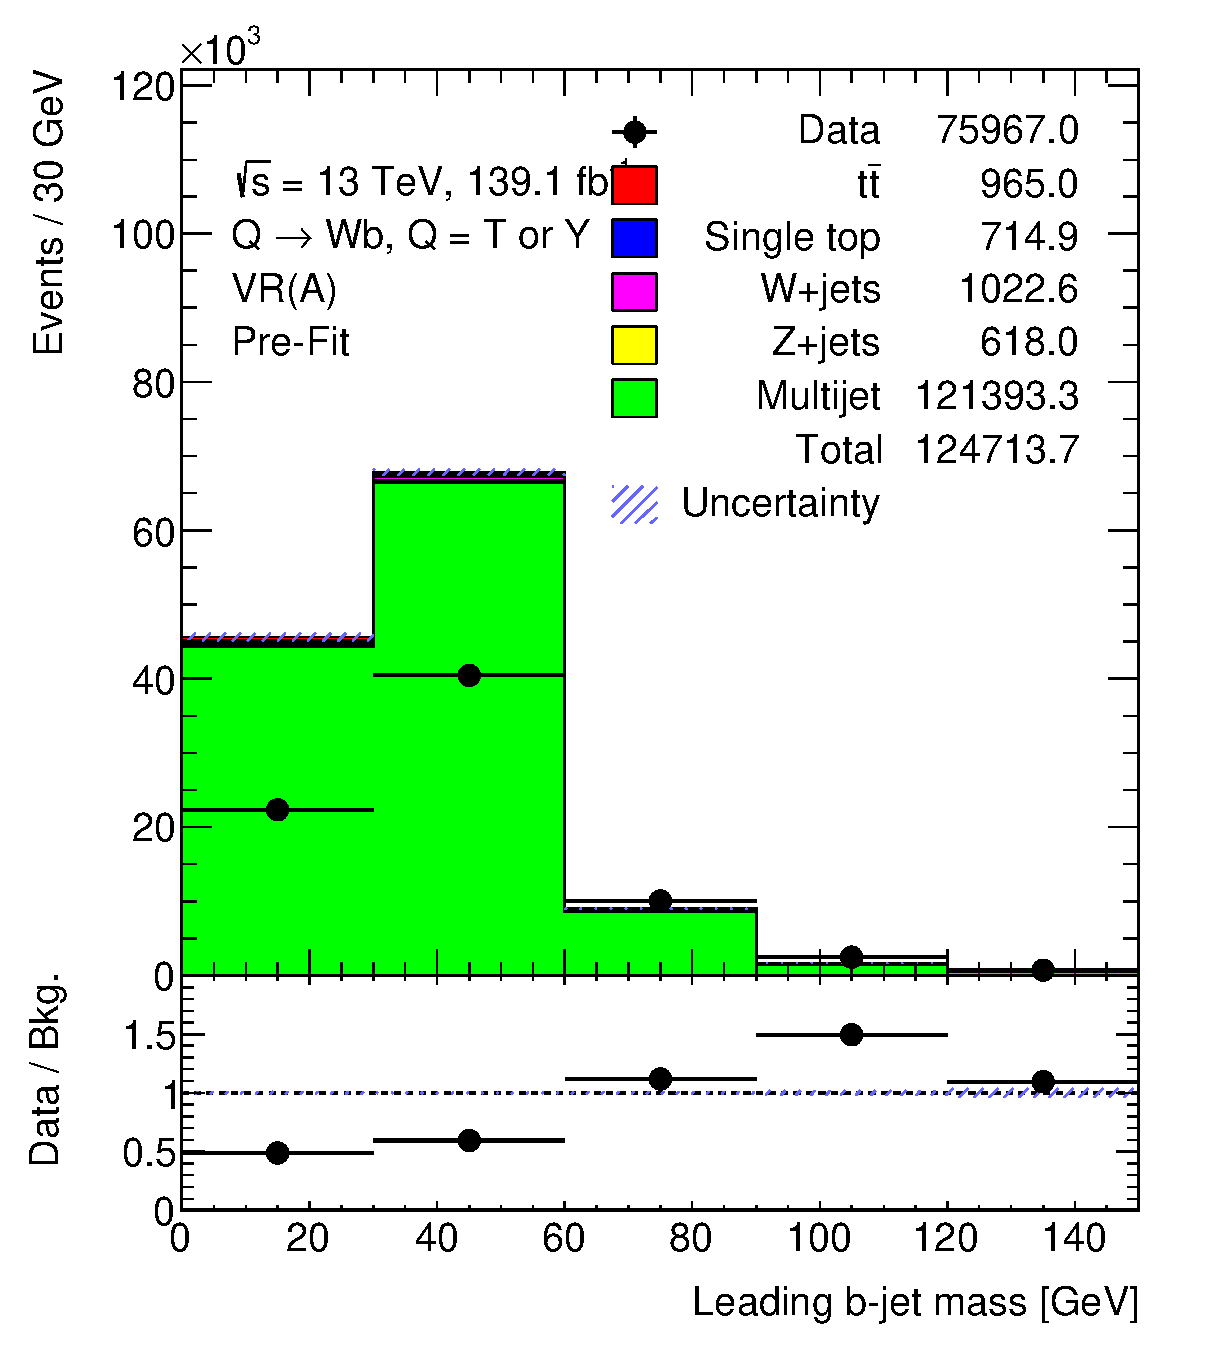
\includegraphics[width=\linewidth,height=\textheight,keepaspectratio]{VR_B_jet_m.eps}
		\caption{}
		\label{fig:abcd:furtherimprovement:scaledcorr:jet_m}
	\end{subfigure}
	\caption{A data/bkg.\ comparison of kinematic and reconstructed variables in VR A where multijet background is estimated from the ABCD method in which \R is calculated by using shape method from the scaled multijet MC. The variables include (a) $p_{\text{T}}$ of $W$-tagged large-$R$ jet, (b) $p_{\text{T}}$ of leading $b$-tagged small-$R$ jet, (c) $\eta$ distribution of $W$-tagged large-$R$ jet, (d) mass of $W$-tagged large-$R$ jet, and (e) mass of leading $b$-tagged small-$R$ jet. Errors shown in the plots are all statistical uncertainty.}
	\label{fig:abcd:furtherimprovement:scaledcorr}
\end{figure}

%%% Local Variables: 
%%% mode: latex
%%% TeX-master: "mythesis"
%%% End: 